\documentclass[a4paper,10pt]{article}

\usepackage[utf8]{inputenc}


\usepackage{subfiles}
\usepackage{microtype}

% Required for inserting images
\usepackage{graphicx}

% Math stuff
\usepackage{amsmath}
\usepackage{amssymb}
\usepackage{amsthm}
\usepackage{mathtools}
\usepackage[bb=stix,scr=boondoxo]{mathalpha}

\usepackage{xspace}

% Color definitions
\usepackage[dvipsnames]{xcolor}

% Handle abbreviations
\usepackage[nolist]{acronym}

% Better algorithm
\usepackage[linesnumbered,ruled,vlined]{algorithm2e}

% Better table
\usepackage{booktabs}
\usepackage[footnotehyper]{nicematrix}
\usepackage{makecell}

% Better reference
\usepackage{hyperref}
\hypersetup{                    % ...like so
  colorlinks,
  linkcolor={green!80!black},
  citecolor={red!70!black},
  urlcolor={blue!70!black}
}
\usepackage{cleveref}

\usepackage{cite}

% TODO
\usepackage{todonotes}

% SVG support
\usepackage[inkscapeversion=1]{svg}

% Charts
\usepackage{pgfplots}
\pgfplotsset{compat=newest}
\usetikzlibrary{patterns}

% Colorblind-safe palette (Tol "bright" scheme)
\definecolor{tolblue}{HTML}{4477AA}
\definecolor{tolred}{HTML}{EE6677}
\definecolor{tolgreen}{HTML}{228833}
\definecolor{tolyellow}{HTML}{CCBB44}

\usepackage{enumitem}

\usepackage{authblk}


\makeatletter
\AtBeginDocument
 {
   \def\ltx@label#1{\cref@label{#1}}%add braces
   \def\label@in@display@noarg#1{\cref@old@label@in@display{#1}}%remove braces
\def\label@in@mmeasure@noarg#1{%
    \begingroup%
      \measuring@false%
      \cref@old@label@in@display{#1}%remove braces for multline, see https://tex.stackexchange.com/q/737204/2388
    \endgroup}%  
 } %
\makeatother
% Name for our protocol
\newcommand{\Protocol}{\ensuremath{\mathsf{PlasmaBlind}}\xspace}
\newcommand{\PlasmaFold}{\ensuremath{\mathsf{PlasmaFold}}\xspace}

% For collaboration
\newcommand{\Pierre}[1]{{\color{orange}$^{\text{Pierre}}$ #1}}
\newcommand{\Winderica}[1]{{\color{blue}$^{\text{Winderica}}$ #1}}

% Compact algorithm names
\newcommand{\Fn}{\ensuremath{\mathcal{F}}\xspace}

\newcommand{\Setup}{\ensuremath{\mathcal{G}}\xspace}
\newcommand{\KeyGen}{\ensuremath{\mathcal{K}}\xspace}
\newcommand{\Prove}{\ensuremath{\mathcal{P}}\xspace}
\newcommand{\Sign}{\ensuremath{\mathcal{S}}\xspace}
\newcommand{\Verify}{\ensuremath{\mathcal{V}}\xspace}
\newcommand{\Commit}{\ensuremath{\mathcal{C}}\xspace}
\newcommand{\Update}{\ensuremath{\mathcal{U}}\xspace}

\newcommand{\Adversary}{\ensuremath{\mathscr{A}}\xspace}
\newcommand{\TrustedParty}{\ensuremath{\mathscr{T}}\xspace}
\newcommand{\Simulator}{\ensuremath{\mathscr{S}}\xspace}
\newcommand{\Extractor}{\ensuremath{\mathscr{E}}\xspace}

% For folding schemes
\newcommand{\NIFS}{\ensuremath{\mathsf{NIFS}}\xspace}
\newcommand{\NIFSSetup}{\ensuremath{\mathsf{\NIFS.\Setup}}\xspace}
\newcommand{\NIFSKeyGen}{\ensuremath{\mathsf{\NIFS.\KeyGen}}\xspace}
\newcommand{\NIFSProve}{\ensuremath{\mathsf{\NIFS.\Prove}}\xspace}
\newcommand{\NIFSVerify}{\ensuremath{\mathsf{\NIFS.\Verify}}\xspace}

\newcommand{\U}{\ensuremath{{\mathbb{U}}}\xspace}
\renewcommand{\u}{\ensuremath{{\mathbb{u}}}\xspace}
\newcommand{\W}{\ensuremath{{\mathbb{W}}}\xspace}
\newcommand{\w}{\ensuremath{{\mathbb{w}}}\xspace}
\newcommand{\cf}{\ensuremath{{\mathsf{cf}}}\xspace}
\newcommand{\ROneCS}{\ensuremath{{\mathsf{CS}}}\xspace}

\newcommand{\PCD}{\ensuremath{\mathsf{PCD}}\xspace}



\newcommand{\PRF}{\ensuremath{\mathsf{PRF}}\xspace}


% For Commitment schemes
\newcommand{\CM}{\ensuremath{\mathsf{CM}}\xspace}
\newcommand{\CMKeyGen}{\ensuremath{\mathsf{\CM.\KeyGen}}\xspace}
\newcommand{\CMCommit}{\ensuremath{\mathsf{\CM.\Commit}}\xspace}
\newcommand{\CMVerify}{\ensuremath{\mathsf{\CM.\Verify}}\xspace}

% For IVC
\newcommand{\IVC}{\ensuremath{\mathsf{IVC}}\xspace}
\newcommand{\IVCSetup}{\ensuremath{\mathsf{\IVC.\Setup}}\xspace}
\newcommand{\IVCKeyGen}{\ensuremath{\mathsf{\IVC.\KeyGen}}\xspace}
\newcommand{\IVCProve}{\ensuremath{\mathsf{\IVC.\Prove}}\xspace}
\newcommand{\IVCVerify}{\ensuremath{\mathsf{\IVC.\Verify}}\xspace}
\newcommand{\Aux}{\ensuremath{{\mathsf{aux}}}\xspace}

% For Decider
\newcommand{\Decider}{\ensuremath{\mathsf{Decider}}\xspace}
\newcommand{\DeciderSetup}{\ensuremath{\mathsf{\Decider.\Setup}}\xspace}
\newcommand{\DeciderKeyGen}{\ensuremath{\mathsf{\Decider.\KeyGen}}\xspace}
\newcommand{\DeciderProve}{\ensuremath{\mathsf{\Decider.\Prove}}\xspace}
\newcommand{\DeciderVerify}{\ensuremath{\mathsf{\Decider.\Verify}}\xspace}

% For Signature
\newcommand{\Sig}{\ensuremath{\mathsf{Sig}}\xspace}
\newcommand{\SigKeyGen}{\ensuremath{\mathsf{\Sig.\KeyGen}}\xspace}
\newcommand{\SigSign}{\ensuremath{\mathsf{\Sig.\Sign}}\xspace}
\newcommand{\SigVerify}{\ensuremath{\mathsf{\Sig.\Verify}}\xspace}

% For Accumulators, vector commitments, and merkle trees
\newcommand{\Acc}{\ensuremath{\mathsf{Acc}}\xspace}
\newcommand{\Accumulate}{\ensuremath{\mathcal{A}}\xspace}
\newcommand{\AccProve}{\ensuremath{\mathsf{\Acc.\Prove}}\xspace}
\newcommand{\AccVerify}{\ensuremath{\mathsf{\Acc.\Verify}}\xspace}
\newcommand{\AccAdd}{\ensuremath{\mathsf{\Acc.\Add}}\xspace}
\newcommand{\AccAccumulate}{\ensuremath{\mathsf{\Acc.\Accumulate}}\xspace}
\newcommand{\AccDelete}{\ensuremath{\mathsf{\Acc.\Delete}}\xspace}

\newcommand{\VecCom}{\ensuremath{\mathsf{VC}}\xspace}
\newcommand{\VecComProve}{\ensuremath{\mathsf{\VecCom.\Prove}}\xspace}
\newcommand{\VecComVerify}{\ensuremath{\mathsf{\VecCom.\Verify}}\xspace}
\newcommand{\VecComUpdate}{\ensuremath{\mathsf{\VecCom.\Update}}\xspace}

\newcommand{\Merkle}{\ensuremath{\mathsf{MT}}\xspace}
\newcommand{\Add}{\ensuremath{\mathsf{\Update^{+}}}\xspace}
\newcommand{\Delete}{\ensuremath{\mathsf{\Update^{-}}}\xspace}
\newcommand{\Modify}{\ensuremath{\mathsf{\Update^{\Huge \mathlarger{\mathlarger{*}}}}}\xspace}
\newcommand{\MerkleSetup}{\ensuremath{\mathsf{\Merkle.\Setup}}\xspace}
\newcommand{\MerkleProve}{\ensuremath{\mathsf{\Merkle.\Prove}}\xspace}
\newcommand{\MerkleVerify}{\ensuremath{\mathsf{\Merkle.\Verify}}\xspace}
\newcommand{\MerkleAdd}{\ensuremath{\mathsf{\Merkle.\Add}}\xspace}
\newcommand{\MerkleDelete}{\ensuremath{\mathsf{\Merkle.\Delete}}\xspace}
\newcommand{\MerkleModify}{\ensuremath{\mathsf{\Merkle.\Modify}}\xspace}

\newcommand{\Params}{\ensuremath{{\mathsf{pp}}}\xspace}
\newcommand{\Trapdoors}{\ensuremath{{\mathsf{td}}}\xspace}
\newcommand{\Srs}{\ensuremath{{\mathsf{srs}}}\xspace} % SRS
\newcommand{\Ck}{\ensuremath{{\mathsf{ck}}}\xspace} % Commitment key
\newcommand{\Pk}{\ensuremath{{\mathsf{pk}}}\xspace} % Public key
\newcommand{\Ak}{\ensuremath{{\mathsf{ak}}}\xspace} % Proving (arguing) key
\newcommand{\Sk}{\ensuremath{{\mathsf{sk}}}\xspace} % Secret key
\newcommand{\Vk}{\ensuremath{{\mathsf{vk}}}\xspace} % Verification key

\newcommand{\negl}{\ensuremath{\varepsilon}\xspace}

\newtheorem{definition}{Definition}

% Data structures
\newcommand{\Address}{\ensuremath{\mathsf{addr}}\xspace}

%% Transaction & UTXO
\newcommand{\Amount}{\ensuremath{\ensuremath{\mathsf{val}}}\xspace}
\newcommand{\Id}{\ensuremath{id}\xspace}
\newcommand{\Tx}{\ensuremath{\mathsf{tx}}\xspace}
\newcommand{\TxShielded}{\ensuremath{\overline{\Tx}}\xspace}
\newcommand{\Utxo}{\ensuremath{\mathsf{utxo}}\xspace}
\newcommand{\In}{\ensuremath{\mathcal{I}}\xspace}
\newcommand{\Out}{\ensuremath{\mathcal{O}}\xspace}
\newcommand{\Nullifier}{\ensuremath{\mathsf{null}}\xspace}
\newcommand{\Nonce}{\ensuremath{\mathsf{nonce}}\xspace}
\newcommand{\Block}{\ensuremath{\mathsf{blk}}\xspace}
\newcommand{\Balance}{\ensuremath{\mathsf{bal}}\xspace}


% block
\newcommand{\block}[1]{\ensuremath{blk_{#1}}\xspace}
\newcommand{\blockhashvalue}[1]{\ensuremath{h_{#1}^{\mathsf{blk}}}}

\newcommand{\Witness}[1]{\textcolor{Cerulean}{#1}}


%% Trees
\newcommand{\Tree}{\ensuremath{T}\xspace}
%%% Transaction tree, accepts a mandatory and an optional argument (subscripts for when the transaction tree is being updated within the IVC)
\NewDocumentCommand\txtree{ m o }{\ensuremath{\Tree_{#1\IfValueT{#2}{,#2}}^\mathsf{tx}}\xspace}
%%% UTXO tree, accepts a mandatory and an optional argument (subscripts for when the transaction tree is being updated within the IVC)
\NewDocumentCommand\utxotree{ m o }{\ensuremath{\Tree_{#1\IfValueT{#2}{,#2}}^\mathsf{utxo}}\xspace}
%%% Signer tree
\NewDocumentCommand\signertree{ m o }{\ensuremath{\Tree_{#1\IfValueT{#2}{,#2}}^\mathsf{signer}}\xspace}
%%% Block tree
\newcommand{\blocktree}[1]{\ensuremath{\Tree_{#1}^\mathsf{blk}}\xspace}
%%% Nullifier tree
\newcommand{\nullifiertree}[1]{\ensuremath{\Tree_{#1}^\mathsf{null}}\xspace}

%% Roots
\newcommand{\Root}{\ensuremath{r}\xspace}
\NewDocumentCommand{\txtreeroot}{ m o }{\ensuremath{\Root_{#1\IfValueT{#2}{,#2}}^\mathsf{tx}}\xspace}
\NewDocumentCommand{\utxotreeroot}{ m o }{\ensuremath{\Root_{#1\IfValueT{#2}{,#2}}^{\mathsf{utxo}}}\xspace}
\newcommand{\blocktreeroot}[1]{\ensuremath{\Root_{#1}^{\mathsf{blk}}}\xspace}
\NewDocumentCommand{\signertreeroot}{ m o }{\ensuremath{r^\mathsf{signer}_{#1\IfValueT{#2}{,#2}}}\xspace}

\NewDocumentCommand{\settledutxotreeroot}{ m o }{\ensuremath{\Root_{#1\IfValueT{#2}{,#2}}^{\mathsf{settledutxo}}}\xspace}

\NewDocumentCommand{\nullifiertreeroot}{ m o }{\ensuremath{r^\mathsf{null}_{#1\IfValueT{#2}{,#2}}}\xspace}

%% Merkle Paths
\newcommand{\Path}{\ensuremath{\varpi}\xspace}
\NewDocumentCommand{\merklepathtxtree}{ m o }{\ensuremath{\Path^\mathsf{tx}_{#1\IfValueT{#2}{,#2}}}\xspace}
\NewDocumentCommand{\merklepathutxotree}{ m o }{\ensuremath{\Path^{\mathsf{utxo}}_{#1\IfValueT{#2}{,#2}}}\xspace}
\newcommand{\merklepathblocktree}[2]{\ensuremath{\Path^{\mathsf{blk}}_{#1,#2}}\xspace}
\newcommand{\merklepathsignertree}[2]{\ensuremath{\Path^{\mathsf{signer}}_{#1,#2}}\xspace}


% signer list, idx of signer in signer list
\NewDocumentCommand{\signerlist}{ m o }{\ensuremath{\mathcal{L}_{#1\IfValueT{#2}{,#2}}^{\mathsf{signer}}}\xspace}
\NewDocumentCommand{\signeracc}{ m o }{\ensuremath{\sigma^{\mathsf{signer}}_{#1\IfValueT{#2}{,#2}}}\xspace}

% signer list
\NewDocumentCommand{\nullifierslist}{ m o }{\ensuremath{\mathcal{L}_{#1\IfValueT{#2}{,#2}}^{\mathsf{null}}}\xspace}


% deposit accumulator
\NewDocumentCommand{\depositacc}{ m o }{\ensuremath{\sigma^{\mathsf{deposit}}_{#1\IfValueT{#2}{,#2}}}\xspace}
\NewDocumentCommand{\depositlist}{ m o }{\ensuremath{\mathcal{L}_{#1\IfValueT{#2}{,#2}}^{\mathsf{deposit}}}\xspace}

% withdrawal list, withdrawal accumulator
\NewDocumentCommand{\withdrawallist}{ m o }{\ensuremath{\mathcal{L}_{#1\IfValueT{#2}{,#2}}^{\mathsf{withdraw}}}\xspace}
\NewDocumentCommand{\withdrawacc}{ m o }{\ensuremath{\sigma^{\mathsf{withdraw}}_{#1\IfValueT{#2}{,#2}}}\xspace}

\NewDocumentCommand{\blockacc}{ m o }{\ensuremath{\sigma^{\mathsf{blk}}_{#1\IfValueT{#2}{,#2}}}\xspace}

% IVC circuits
\newcommand{\ivccircuit}[2]{\ensuremath{\Fn^{\mathsf{#1}}_{\mathsf{#2}}}\xspace}

% functions
% \newcommand{\computetxidx}{\ensuremath{\mathtt{idx}(\text{tx})}\xspace}
% \newcommand{\preparetrees}{\ensuremath{\mathtt{PrepareTrees}}\xspace}
% \newcommand{\signsend}{\ensuremath{\mathtt{SignSend}}\xspace}
% \newcommand{\sign}[1]{\ensuremath{\mathtt{sign(}#1\mathtt{)}}}

% IVC proofs
\newcommand{\ivcbalanceproof}[1]{\ensuremath{\pi_{#1}}\xspace}
\newcommand{\ivcblockproof}[1]{\ensuremath{\Pi_{#1}}\xspace}


% Algorithm
%% keywords
\SetKwProg{Function}{Function}{:}{}
\SetKwProg{Circuit}{Circuit}{:}{}
\SetKw{Enforce}{enforce}{}
%% Comment starting with a triangle
\SetKwComment{Comment}{$\triangleright$\ }{}
\newcommand\CommentStyle[1]{\rmfamily{#1}}
\SetCommentSty{CommentStyle}

% Math
\newcommand{\concat}{\ensuremath{\mathbin\Vert}}
\renewcommand{\vec}[1]{\boldsymbol{#1}}
\newcommand{\mat}[1]{\boldsymbol{#1}}
%% A short hyphen in math mode
\mathchardef\mhyphen="2D
%% Better \emptyset
\let\oldemptyset\emptyset
\let\emptyset\varnothing


\newcommand{\IVLS}{\ensuremath{\mathsf{IVLS}}\xspace}


\newcommand{\sonobe}{\texttt{Sonobe}}
\newcommand{\arkworks}{\texttt{Arkworks}}
\newcommand{\implementationurl}{\url{https://github.com/dmpierre/plasma-fold}}


\title{\Protocol: A Private Layer 2 With \\ Instant Client-Side Proving}
\author[1]{Pierre Daix-Moreux}
\author[1,2]{Chengru Zhang}
\affil[1]{Ethereum Foundation}
\affil[2]{The University of Hong Kong}
\affil[ ]{\url{pierre@ethereum.org}, \url{u3008875@connect.hku.hk}}
\date{}

\newtheorem{construction}{Construction}

\begin{document}

\begin{acronym}
    \acro{p.p.t.}{Probabilistic Polynomial Time}
    \acro{NIFS}{non-interactive folding scheme}
    \acro{IVC}{Incrementally Verifiable Computation}
    \acro{PCD}{Proof-Carrying Data}
    \acro{zk}{zero-knowledge}
    \acro{SNARK}{Succinct Non-Interactive Argument of Knowledge}
    \acro{zkSNARK}{Zero-Knowledge Succinct Non-Interactive Argument of Knowledge}
    \acro{TPS}{transactions per second}
    \acro{UTXO}{Unspent Transaction Output}
    \acro{L1}{Layer-1}
    \acro{L2}{Layer-2}
    \acro{R1CS}{Rank-1 Constraint System}
    \acro{RR1CS}{Relaxed R1CS}
    \acro{AZTEC}{Anonymous Zero-Knowledge Transactions with Efficient Communication}
    \acro{DSL}{Domain-Specific Language}
\end{acronym}


\maketitle

\begin{abstract}

In this technical note, we discuss a new direction in the design of privacy-preserving and scalable \ac{L2} protocols by presenting a concrete construction, \Protocol.

To minimize the \ac{L2} users' overhead for achieving privacy while enabling efficient creation of compact blocks, \Protocol is built upon a novel architecture that leverages folding schemes' powerful and flexible properties.
On the user side, we utilize their \textit{blinding} property to shield and prove transaction data without expensive succinct zero-knowledge proofs.
On the aggregator side, their \textit{low accumulation cost} allows efficient aggregation of user instances into a constant size proof of block validity.


We further improve our proof aggregation performance by proposing an optimization technique that efficiently links two different verification tasks with shared input while eliminating the need for cumbersome proof composition of non-uniform circuits, which could be of independent interest.

The practicality of \Protocol is validated by our preliminary benchmarks, which demonstrate that, with consumer hardware, \Protocol achieves sub-100ms proving time on the client side and sub-300ms per-transaction time on the aggregator side.

\end{abstract}

\section{Introduction}

Public blockchains suffer from two well-known limitations: low throughput~\cite{FCW:CDEGJK16} and lack of privacy~\cite{FC:RonSha13}.
Their limited throughput is due to the requirement that every validator independently re-executes every transaction, bounding the chain's processing capacity by that of a single node.
Their lack of privacy is the result of recording all transactions on a public ledger in plaintext.
Even though the real-world identities of senders and recipients are obfuscated by addresses, they can be revealed through transaction graph analysis and exchange data correlation, offering only pseudonymity rather than full anonymity.

Two largely independent lines of research have sought to address these limitations.

On the \textit{scalability} front, \ac{L2} protocols offload transaction processing from the base \ac{L1} blockchain to an off-chain aggregator that batches transactions and posts compressed updates on-chain.
However, these designs offer no privacy: even when compressed block data reveals only limited information to external observers, the aggregator has full visibility into every transaction.
For example, validity rollups, often called ``zk-rollups'', use \acp{zkSNARK} only to prove the correctness of state transitions; the ``zero-knowledge'' qualifier refers to the succinctness of the validity proof, not to any privacy guarantee.

On the \textit{privacy} front, protocols such as Zerocoin~\cite{SP:MGGR13}, Zerocash~\cite{SP:BCGGMT14}, and subsequent works demonstrated how zero-knowledge proofs, especially \acp{zkSNARK}, can hide transaction contents while ensuring honest behaviors by having users generate proofs of transaction validity.
However, these protocols typically deploy as standalone \acp{L1}, inheriting the base layer's throughput constraints.
For instance, ZCash, the deployed implementation of Zerocash, achieves $<$10 \ac{TPS}\footnote{\url{https://phemex.com/academy/what-is-zcash-zec}}.

Recent work has attempted to combine privacy with scalability by shielding (hiding) transactions on \acp{L2}.
However, existing approaches impose a large computational burden on either the user or the aggregator.
Nightfall~\cite{nightfall4} supports shielded transactions on an \ac{L2} but suffers from huge aggregator proving costs, requiring a machine with 144 cores and 750\,GB RAM to build blocks of just 64 transactions.
Intmax2~\cite{cryptoeprint:2023/1082} has high theoretical throughput thanks to their block compression technique via short user identifiers and client-side proving.
However, they require the senders to prove their transaction history and the recipients to merge the sender's proof with their own transaction history using heavy cryptographic primitives for proof composition.
It is also mandatory for users to synchronize their proofs for \textit{every} block even if it does not contain relevant transactions, limiting practical usability.

In this technical note, we therefore study the following question:

\begin{center}
    \textit{Can we design a private and scalable \ac{L2} \\ without sacrificing efficiency on both the user and aggregator sides?}
\end{center}

We provide a novel solution to this question by extending PlasmaFold~\cite{cryptoeprint:2025/1300} and presenting \Protocol.
\Protocol achieves privacy of transaction amounts and recipients and enables high throughput, all while maintaining low proof generation costs for both users and aggregators.
Furthermore, users in \Protocol enjoy fast synchronization and instant exits.

Below we elaborate on the key features of our construction.

\paragraph{Transaction privacy with efficient client-side proving.}
\Protocol operates in the \ac{UTXO} model and provides transaction privacy by hiding transaction amounts and recipients in shielded transactions.
Although users must generate zero-knowledge proofs attesting to the validity of these transactions, we minimize the computational burden for proof generation.
Instead of requiring users to run an expensive \ac{zkSNARK} prover, we leverage the blinding property of folding schemes and utilize the BlindFold~\cite{C:KotSet24} technique.
This allows users to prove transaction validity by simply rerandomizing a satisfying instance-witness pair via folding, which takes less than 100ms on consumer hardware and is practical for a wide range of users.

\paragraph{Optimized proof aggregation.}
We design a tailored \ac{L2} aggregator who is able to prove \ac{L2} state updates \textit{while} aggregating users' transaction validity proofs.

A naive but inefficient approach would be to use a \ac{PCD} scheme to combine the local execution (i.e., state updates) with the external proofs (i.e., transaction validity proofs) and take care of the non-uniformity of the circuits for these tasks.

We instead propose a more efficient architecture that avoids the need for non-uniform \ac{PCD}, where we decompose this workload into two uniform \ac{IVC} chains while designing an augmented circuit that ensures the two chains are linked by a shared transaction.
The performance is further boosted by the low accumulation cost of folding schemes.
By using folding-based \ac{IVC}, our aggregators are able to achieve sub-300ms time for handling each transaction (and its associated proof).

\paragraph{Scalable and trust-minimized block building.}

The architecture of our proof aggregation enables scalable block building with minimal trust assumptions on the aggregator.

First, our design guarantees that the validity of all blocks are enforced by cryptographic proofs, eliminating the need for a fraud proof mechanism or trust assumptions on the aggregator's honesty.
The final block validity proof is constant in size regardless of the number of aggregated proofs, and combining it with the short ID design from Intmax2 \cite{cryptoeprint:2023/1082}, we can achieve high scalability with minimal on-chain data posting.

Second, thanks to our emulation of \ac{PCD} using \ac{IVC}, \Protocol not only supports a single, permissioned aggregator building blocks by sequentially folding user proofs, but also allows multiple permissionless aggregators to aggregate user proofs in parallel.

\paragraph{Instant exits and fast synchronization.}

In \Protocol, we further leverage balance proofs maintained by users, enabling instant exits from the \ac{L2} at any time, without revealing their transaction history or interacting with the aggregator.

However, to achieve fast synchronization, we improve the design of balance proofs in two aspects.
First, balance proofs are efficiently updated via folding-based \ac{IVC} using \ac{L2}'s latest state, which is already attested by the aggregator's proof.
This is in contrast to Intmax2 \cite{cryptoeprint:2023/1082}, where transaction state is maintained by users and updated via costly \ac{PCD} routines.
Second, our combination of a Merkle tree of blocks and balance proofs allows users to skip synchronization for blocks that contain no relevant transactions to them, who only need to update their balance proofs when they send or receive transactions.

\section{Overview of \Protocol}\label{sec:overview}


In this section, we provide a high-level overview of \Protocol via a progression of increasingly refined constructions.
Starting from a naive \ac{L2} design, we identify shortcomings and address them step by step, introducing the cryptographic tools that motivate our final protocol along the way.

\paragraph{Strawman 1: a naive design with scalability and privacy.}
We consider an \ac{L2} construction that naively combines existing scalability and privacy solutions.
In this setting, there are many users on the \ac{L2} who wish to transact with each other, and a rollup contract on the \ac{L1} that enforces the correctness of the \ac{L2} state.

For scalability, an \textit{aggregator} collects transactions from users, assembles them into compressed \textit{blocks}, and submits each block to the rollup contract.
Different design families, such as rollups, plasma, and validium, vary in their data availability and security tradeoffs, but in all cases the aggregator must additionally demonstrate that the new state digest faithfully reflects the execution of all transactions in the block, either via a fraud proof or a validity proof.

For privacy, users send \textit{shielded transactions} whose contents are hidden instead of their plaintext transaction data.
Each shielded transaction must be accompanied by a zero-knowledge proof of transaction validity (i.e., that the sender owns the spent funds, no double-spending occurs, etc.) without revealing amounts or participants.
The use of zero-knowledge proofs for cryptocurrencies was pioneered by Zerocoin~\cite{SP:MGGR13}. It was later refined by Zerocash~\cite{SP:BCGGMT14} and subsequent works~\cite{AC:FMMO19,FC:BAZB20,SP:Diamond21,ESORICS:ChaBal21,ASIACCS:CamHal22,SP:GKPH24,AC:MadSca25,EPRINT:SKKK25} in terms of efficiency and functionality.

In these protocols, transactions are defined within two main models: the \textit{UTXO-based model} and the \textit{account-based model}.
This work focuses on the \ac{UTXO}-based model, where each (transparent) transaction consumes existing \acp{UTXO} and creates new ones.
To shield such transactions, consumed \acp{UTXO} are replaced by \textit{nullifiers}, which are unique, deterministic tags that prevent double-spending without revealing which output is consumed.
In addition, created output \acp{UTXO} are replaced by cryptographic \textit{commitments} binding to the amounts and recipients while hiding their concrete values.

On the other hand, the account-based model defines transactions as updates to account balances.
A typical approach to hiding transactions in this model is proposed in (Anonymous) Zether~\cite{FC:BAZB20}, where balances are encrypted and homomorphically updated by each transaction.
However, this approach leaks transaction patterns and requires computational overhead at least linear in the anonymity set to mitigate them.

To efficiently prove that a transaction is consistent with the current \ac{L2} state, the rollup contract maintains a succinct state digest via a \textit{cryptographic accumulator}~\cite{EC:BendMa93} (e.g., Merkle trees~\cite{C:Merkle87} or RSA accumulators~\cite{EC:BarPfi97}), allowing users to generate proofs against the on-chain digest without accessing the entire state.

While Strawman 1 achieves both privacy and scalability in principle, two practical bottlenecks remain.
First, generating transaction validity proofs typically requires a general-purpose \ac{zkSNARK} prover for circuit satisfiability~\cite{EC:Groth16,EPRINT:GabWilCio19}, which incurs high computational cost on the client side.
Second, the aggregator must aggregate all transaction validity proofs into a single block validity proof, which remains costly even with existing techniques such as SnarkPack~\cite{FC:GaiMalNit22}.
These bottlenecks are evident in deployed systems: for example, the \ac{AZTEC} protocol suffers from high aggregation costs (60 GB of RAM) and low throughput (0.2 TPS in their testnet) \footnote{\url{https://blog.zkcloud.com/p/what-does-it-take-to-prove-aztecs}}.
Similarly, Nightfall~\cite{nightfall4} requires 144 CPU cores and 750GB of RAM to build blocks composed of 64 transactions.

\paragraph{Strawman 2: utilizing proof composition.}

A standard technique to reduce the cost of proof aggregation is to use \ac{IVC}~\cite{TCC:Valiant08} and \ac{PCD}~\cite{ITCS:ChiTro10}.
\ac{IVC} allows a prover to repeatedly apply a fixed step function to an evolving state and produce a proof that the entire chain of computations is correct, regardless of the number of steps.
\ac{PCD} generalizes this to distributed computations with a tree-like or DAG-shaped structure, where multiple independent provers contribute proofs that can be recursively composed into a single proof.

Applied to our setting, the aggregator can use \ac{IVC} or \ac{PCD} to incrementally incorporate user proofs as they arrive, rather than waiting for the entire block before starting aggregation.
Moreover, each composition step typically incurs a low recursive overhead, making it much cheaper than the brute-force approach of naively encoding the entire proof verification algorithm as a circuit.

However, two issues remain with this approach.
First, users must still generate a (zero-knowledge) \ac{IVC} or \ac{PCD} proof on the client side, which imposes computational overhead and is impractical for users with limited hardware resources.
Second, achieving high throughput requires the aggregator to maintain a stateful architecture in which it must prove both the validity of user proofs \textit{and} the correctness of \ac{L2} state transitions.
This can be abstracted as the task of generating a proof that attests to both local execution and external proof verification at each step, naturally leading to a tree-like computation structure that \ac{IVC} (which only supports linear composition) cannot express, thus requiring the more general but expensive \ac{PCD} machinery.
The problem is further compounded by the fact that local execution (\ac{L2} state updates) and external proof verification (transaction validity) involve circuits of different shapes, resulting in \textit{non-uniform} computation that makes the \ac{PCD} even more costly.

Some constructions, such as Intmax2, further push the idea of proof composition to the client side to minimize the aggregator's workload. However, this exacerbates the first issue by requiring users to generate even more complex proofs.
Specifically, users in Intmax2 are responsible for maintaining their transaction state, and when the sender transfers funds to a recipient, the sender must generate a proof showing the transaction history behind the funds is valid.
Also, the recipient needs to use \ac{PCD} to combine the sender's proof with their own proof of transaction history and obtain an updated proof of the new transaction state.

\paragraph{Final construction: maximizing efficiency with folding.}

We take a different approach and address both issues by leveraging \textit{folding schemes}~\cite{C:KotSetTzi22}.
A folding scheme allows two instance-witness pairs for the same circuit to be ``folded'' into a single pair that remains satisfying, and this folding operation is much cheaper than generating a full proof.

A key observation in~\cite{C:KotSet24} is that some folding schemes are \textit{blinding}: when a satisfying instance-witness pair is folded with a uniformly random pair, the result reveals no information about the original witness.
This property can be utilized to make client-side proving more efficient.
A user who holds a satisfying witness of the transaction validity circuit simply folds it with a fresh random pair; the output serves as a zero-knowledge proof of knowledge of the original witness, without ever invoking a full \ac{zkSNARK} or zero-knowledge \ac{IVC} prover.
This directly resolves the first issue from Strawman 2: users only evaluate the transaction validity circuit and perform a single folding step, achieving much lower client-side proving costs.

To resolve the second issue of Strawman 2, we design a proof aggregation architecture that avoids naive non-uniform \ac{PCD}.
The core idea is to decompose the aggregator's workload into two independent but linked \ac{IVC} chains, each with a \textit{uniform} step function.
The first chain handles user proof aggregation: upon receiving a transaction validity proof (a rerandomized instance-witness pair), the aggregator folds it into a running accumulated pair.
The second chain handles \ac{L2} state updates: the aggregator executes the state transition circuit for the corresponding transaction and folds the witness-instance pair for the execution into a separate running accumulated pair.
To ensure consistency between the two chains, the state update circuit is augmented to verify that the user proof folded in the first chain corresponds to the \textit{same transaction} used for the state update in the second chain.
This linking mechanism ties the two uniform \ac{IVC} chains together, achieving the expressiveness of non-uniform \ac{PCD} without its overhead.

As an additional benefit, folding schemes enable instant exits for users.
When a user wishes to exit the \ac{L2} and withdraw their funds back to the \ac{L1}, they need to provide a proof of their current balance.
Instead of generating the proof from scratch when exiting, users can locally maintain a balance proof and efficiently update the proof after each transaction by using folding-based IVC.

As a concrete instantiation, we present \Protocol, which realizes the above design in the \ac{UTXO} model.
Built upon \PlasmaFold~\cite{cryptoeprint:2025/1300}, which combined Intmax2's on-chain data minimization with folding-based \ac{IVC} for efficient aggregation in a non-private setting, \Protocol further adds sender-receiver unlinkability and confidentiality of transaction amounts by utilizing the Nova folding scheme~\cite{C:KotSetTzi22} and its BlindFold extension~\cite{C:KotSet24} for efficient client-side proving and proof aggregation.
Nova achieves support for \ac{R1CS} witnesses and instances by introducing a variant, the committed relaxed \ac{R1CS}, where a satisfying witness-instance pair $(\W = (w, e, r_w, r_e), \U = (\overline{w}, \overline{e}, u, x))$ must satisfy the R1CS structure $A, B, C$ if $A z \circ B z - C \cdot z = e$ for $z = (u, x, w)$, and $\overline{w}$ and $\overline{e}$ must be commitments to $w$ and $e$ with randomness $r_w$ and $r_e$ respectively.
The original R1CS witness-instance pair $(\w = w, \u = x)$ can thus be regarded as a special case of the committed relaxed R1CS with $u = 1$ and $e = 0$.

In an interactive setting of Nova, a prover and a verifier fold two witness-instance pair $(\W_1 = (w_1, e_1, r_{w_1}, r_{e_1}), \U_1 = (\overline{w}_1, \overline{e}_1, u_1, x_1))$ and $(\W_2 = (w_2, e_2, r_{w_2}, r_{e_2}), \U_2 = (\overline{w}_2, \overline{e}_2, u_2, x_2))$ as follows.
The prover computes $z_i = (u_i, x_i, w_i)$ and sends to the verifier a commitment $\overline{t}$ to the cross-term $t = A z_1 \circ B z_2 + A z_2 \circ B z_1 - u_1 C z_1 - u_2 C z_2$ with randomness $r_t$, and the verifier responds with a random challenge $\rho$.
Then both parties compute the folded instance $\U$ as $\overline{w} = \overline{w}_1 + \rho \overline{w}_2, \overline{e} = \overline{e}_1 + \rho \overline{t} + \rho^2 \overline{e_2}, u = u_1 + \rho u_2, x = x_1 + \rho x_2$.
The prover further computes the folded witness $\W$ as $w = w_1 + \rho w_2, r_w = r_{w_1} + \rho r_{w_2}, e = e_1 + \rho t+ \rho^2 e_2, r_e = r_{e_1} + \rho r_t + \rho^2 r_2$.

By observing that Nova is a blinding folding scheme, NovaBlindFold achieves zero-knowledge by folding a satisfying instance-witness pair $(\w, \u)$ with a randomly sampled $(\W^\$, \U^\$)$.
The folded witness $\W$ does not reveal any information about $\w$, while the satisfiability of $\w$ and $\u$ can be verified by folding $\u$ and $\U^\$ $ and checking that $\W$ and the resulting $\U$ are satisfying.


\Protocol further adopts Intmax2's~\cite{cryptoeprint:2023/1082} data availability and block compression design to minimize data posted on-chain.
In this design, one round of interaction between the aggregator and the sender is required.
Having received a shielded transaction from a sender, the aggregator needs to first return a \textit{receipt} containing \ac{L2} state relevant to the transaction (Merkle proofs in our case).
Only after this will the sender reply with an \textit{endorsement} (transaction validity proofs in our case), without which the aggregator cannot include the transaction in a block.


\section{Construction of \Protocol}

As an efficient and scalable \ac{L2} protocol for private transactions, \Protocol specifies the interactions among three types of parties: the \textit{user}, the \textit{aggregator}, and the \textit{rollup contract}.
To introduce the construction of \Protocol, we first recap its high-level design introduced in~\Cref{sec:overview}, and then we elaborate on the specific data structures and behaviors of each party.

When a user (sender) makes a transfer to another user (recipient), the sender builds a \textit{transparent transaction} for the transfer and converts it to a \textit{shielded transaction} by hiding its content.
The shielded transaction is then sent to the aggregator.

We then leverage Intmax2's idea that ensures data availability using interaction between the sender and the aggregator.
After collecting transactions from all senders, the aggregator builds a \textit{Merkle tree} on top of the transactions and returns to each sender a \textit{Merkle proof} as the \textit{receipt}.

At this point, all transactions are regarded as unsettled.
Every sender needs to provide the aggregator with an \textit{endorsement}, instantiated as the \textit{transaction proof} attesting to their transaction validity, to settle their transactions upon receiving the receipt.

Next, the aggregator builds a \textit{block} for transactions with valid proofs, accumulates all valid proofs into a short \textit{block proof}, and proposes the block to the rollup contract.
The rollup contract verifies the attached block proof and updates the \textit{nonces} for senders with endorsed transactions.

Furthermore, senders and recipients use the receipt and onchain data to update their local \textit{balance proofs}, which are useful when the user wishes to non-interactively withdraw funds from the L2.

\subsection{Notions and Data Structures}

We now list the notions and data structures involved in \Protocol.
For each notion or data structure, we explain its purpose and discuss how it is constructed and maintained by \Protocol participants.

\subsubsection{Keys}

Every user in \Protocol has a secret key $\Sk$ and a public key $\Pk$.
$\Pk$ represents the user's identity in \Protocol, while $\Sk$ is used to authorize transactions, ensuring that funds can only be spent by their owners.

Upon joining \Protocol, every user needs to create a key pair $(\Sk, \Pk)$, submit the public key $\Pk$ to the rollup contract, and store the secret key $\Sk$ locally.
The contract appends \Pk to a mapping of public keys maintained in its state.

When sending funds to other users, the sender must generate a proof showing that the public key \Pk associated with the funds is indeed derived from the sender's secret key \Sk.
Looking ahead, while a classic signature scheme such as ECDSA could be used, we instead opt for a general-purpose zero-knowledge proof to demonstrate the knowledge of \Sk, which is more flexible and can be easily composed with other proofs.

To maximize the efficiency of this general-purpose proof, we further note that \Protocol is a separate \ac{L2} protocol built upon the \ac{L1}.
Thus, it is not necessary for $\Sk$ and $\Pk$ to have the same format as the \ac{L1}'s secret-public key pairs (e.g., be based on elliptic curves).
Consequently, we can simply derive \Pk from \Sk as $\Pk \coloneqq \PRF(\Sk, \bot)$ using a PRF based on a circuit-friendly hash function.

\subsubsection{Nonces}

A nonce \Nonce in \Protocol is an increment-only counter that tracks the total number of transactions sent by a user.
It is stored by both the user and the rollup contract and is updated whenever a new transaction sent by the user is verified.

The purpose of \Nonce is to prevent users from omitting expenditures from their balance proofs.
Specifically, a malicious user may skip updating their balance proof after spending some funds and later claim a higher balance than they actually have when exiting \Protocol.
In our solution, we require the user to submit their local nonce to the rollup contract when exiting, which will be compared with the latest nonce stored onchain.
The user cannot arbitrarily set their local nonce, since we use the balance proof to guarantee that the local nonce can be incremented only when the user updates their balance with an expenditure.

\subsubsection{Transactions}

\Protocol operates in the \ac{UTXO} model, and a transaction in \Protocol consumes old \acp{UTXO} to create new \acp{UTXO}.
A \ac{UTXO} is denoted as $\Utxo \coloneqq (\Pk, \Amount)$, where \Amount and \Pk are respectively the \ac{UTXO}'s value and the public key of the \ac{UTXO}'s owner.

We consider two forms of transactions: \textit{transparent transactions} and \textit{shielded transactions}, as defined below.

\paragraph{Transparent transactions.}
A transparent transaction contains the consumed input \acp{UTXO} and the created output \acp{UTXO} in plaintext.
It is only known to the sender for privacy of transaction data such as recipients and amounts, and is never shared with the aggregator or other users.
Formally, a transparent transaction with $m$ input \acp{UTXO} and $n$ output \acp{UTXO} is defined as $\Tx \coloneqq (\{ \Utxo^\In_i \}^{m - 1}_{i = 0}, \{ \Utxo^\Out_j \}^{n - 1}_{j = 0})$.

\paragraph{Shielded transactions.}
Instead of transparent transactions, shielded transactions are what users send to the aggregator and their peer users in \Protocol.
They are derived from transparent transactions by hiding the input \acp{UTXO} with \textit{nullifiers} and the output \acp{UTXO} with \textit{committed \acp{UTXO}}.
Formally, a shielded transaction with $m$ input nullifiers and $n$ output \acp{UTXO} is defined as $\TxShielded = (\{ \Nullifier^\In_i \}^{m - 1}_{i = 0}, \{ \overline{\Utxo}^\Out_j \}^{n - 1}_{j = 0})$.

\begin{itemize}
    \item \textit{Nullifiers.}
    A nullifier $\Nullifier$ signifies the consumption of a \ac{UTXO}.
    For a transaction sender to spend a \ac{UTXO} that they have received previously, 
    they must provide the \ac{UTXO}'s corresponding nullifier, which must not exist in the set of all previous nullifiers.
    We require that each \ac{UTXO} has a unique nullifier, and that the nullifier does not leak information about the \ac{UTXO}.
    In this way, the sender is prevented from double-spending, while anyone other than the sender cannot learn the sender's transaction history.

    To achieve both requirements, we utilize a collision-resistant \PRF to deterministically derive the nullifier from the sender's secret key \Sk and the \ac{UTXO}'s position.
    Specifically, suppose the sender owns a previously received \ac{UTXO}, which is the $j$-th output of the $k$-th transaction at the $t$-th block.
    Now, to spend this \ac{UTXO}, the sender derives the corresponding nullifier $\Nullifier \coloneqq \PRF(\Sk, (j, k, t))$.
    Intuitively, every \ac{UTXO} can be uniquely identified by its position $(j, k, t)$, and consequently there is only one nullifier that corresponds to a specific \ac{UTXO} owned by a specific user.
    On the other hand, collision resistance ensures that it is computationally infeasible to find two different pairs of secret keys and positions that yield the same nullifier, which prevents the adversary from spending others' \acp{UTXO}.
    Furthermore, the confidentiality of \ac{UTXO} is guaranteed because the output of \PRF is indistinguishable from a truly random string.

    \item \textit{Committed \acp{UTXO}.}
    A committed \ac{UTXO} $\overline{\Utxo}$ is a commitment to a \ac{UTXO} $\Utxo$.
    More specifically, we compute $\overline{\Utxo} \coloneqq \CMCommit(\Ck, \Utxo; \rho)$ using a commitment scheme $\CM$ under commitment key $\Ck$ and opening $\rho$. 
    
    Committed \acp{UTXO} are submitted to the aggregator to signify the creation of new \acp{UTXO}, while their values and recipients are kept secret due to the hiding property of $\CM$.
    In addition, openings need to be sent to the corresponding recipients, so that they can later claim the ownership of their received \acp{UTXO}, and the binding property of $\CM$ ensures the commitments are opened to the correct values.
\end{itemize}

\subsubsection{Blocks and trees}

A block in \Protocol is a summary of transaction data proposed by the aggregator in a specific period of time.
While an intuitive design is to record every piece of transaction information in blocks, we leverage Merkle trees $\Tree$ (or vector commitments in general) to reduce calldata size and onchain storage.
Specifically, we record succinct digests (i.e., Merkle roots $\Root$) of transaction information in the rollup contract's state, and require the user and the aggregator to demonstrate the validity of Merkle proofs $\Path$ against the onchain roots when making transactions or proposing blocks, thereby preventing them from maliciously claiming or manipulating transaction data.

The following types of Merkle trees are involved in \Protocol:

\begin{enumerate}
    \item \textit{Committed \ac{UTXO} tree.}
    A committed \ac{UTXO} tree $\Tree^{\overline{\Utxo}}_t$ is an ephemeral data structure specific to the block at height $t$.
    It is maintained by the aggregator and contains committed \acp{UTXO} of all \textit{unsettled} shielded transactions in the block as leaves.
    We stress that $\Tree^{\overline{\Utxo}}_t$ is for unsettled \acp{UTXO}.
    In other words, while these committed UTXOs are contained in the tree, they may not indicate the consumption of old \acp{UTXO} and the creation of new \acp{UTXO}, 
    because it is still unknown whether they will be endorsed when building the committed \ac{UTXO} tree.
    \item \textit{Public key tree.}
    A public key tree $\Tree^\Pk_t$ is an ephemeral data structure specific to the block at height $t$.
    It is maintained by the aggregator and contains either the sender's public key of the corresponding transaction in the block or $\bot$, depending on whether the sender has successfully demonstrated the validity of their transaction by providing a transaction proof (introduced later).
    \item \textit{Nullifier tree.}
    The nullifier tree $\Tree^\Nullifier$ is a permanent, global data structure.
    It is maintained by the aggregator, who computes \ac{IVC} proofs attesting to root transitions, and contains all historical valid nullifiers as leaves. The rollup contract stores the latest root and updates it upon receiving a valid proof.
    \item \textit{Block tree.}
    The block tree $\Tree^\Block$ is a permanent, global data structure.
    It is maintained by the aggregator and contains the header (introduced later) of every historical valid block as leaves.
    A copy of the block tree is also stored by the rollup contract, which only verifies the root transition but does not update the tree itself.
\end{enumerate}

In addition to the syntax introduced above, we further use $\Tree_{[i]}$ (resp. $\Root_{[i]}$) for $i \in [0, m]$ to denote the intermediate Merkle tree (resp. root) that already contains $i$ leaves and will eventually have $m$ leaves.
Hence, $\Tree = \Tree_{[m]}$ (resp. $\Root = \Root_{[m]}$) can be considered as the shorthand for the final tree (resp. root).

We subsequently define a block $\Block_t$ at height $t$ by splitting it into two parts: the header $\mathsf{header}$ and the body $\mathsf{body}$.

$\mathsf{header}$, recorded by the rollup contract, contains the committed \ac{UTXO} tree root $\Root^{\overline{\Utxo}}_t$,
the public key tree root $\Root^\Pk_t$,
and the nullifier tree root $\Root^\Nullifier_{[t]}$,
% and the block tree root $\Root^\Block_{[t]}$,
which are short enough for efficient hash computation of block tree leaves and low onchain storage overhead.

On the other hand, $\mathsf{body}$ includes extra information that is necessary to prevent the aggregator from misbehaving.
Although most of transaction data, such as nullifier values, can be locally maintained by the aggregator, it is sometimes inevitable to publish part of transaction data.
For instance, the aggregator may (deliberately or accidentally) ignore a user's transaction by inserting $\bot$ into the public key tree, even if the user has provided a valid transaction proof.
Thus, in line with Intmax2's setup, we require the aggregator to post onchain the leaves of $\Tree^\Pk_t$, so that users can learn whether the aggregator has included their transactions in the current block.
This information will also be used by the rollup contract to update users' nonces.
Fortunately, we can avoid storing $\mathsf{body}$ as the rollup contract's state.
This is because when invoking the rollup contract on input $\Block$, $\mathsf{body}$ is a part of the calldata, which can be later retrieved from full nodes.


\subsubsection{Proofs}

Proofs are crucial components in \Protocol, which enforce that our users and aggregator behave correctly.
We consider three types of proofs:

\begin{enumerate}
    \item \textit{Transaction proofs.}
    Recall that, to ensure the confidentiality of transaction data such as recipients and amounts, users in \Protocol send shielded transactions containing nullifiers and committed \acp{UTXO}.
    Consequently, the aggregator cannot learn the original input or output \acp{UTXO} and is unable to check whether users' transactions are valid.
    Instead, it is the sender's responsibility to show the validity of their submitted shielded transactions.
    
    To this end, the sender generates a \textit{transaction proof} $\pi^\Tx$ that witnesses $w = (\Sk, \Tx)$ and public inputs $x = (\Pk, \TxShielded, \Root^\Block)$ satisfy the transaction validity relation $R^\Tx$.

    Informally, $R^\Tx$ holds if and only if:
    \begin{itemize}
        \item $\Pk$ is correctly derived from $\Sk$.
        \item For every input \ac{UTXO} $\Utxo^\In_i$ in $\Tx$:
        \begin{itemize}
            \item $\Pk$ is the owner of $\Utxo^\In_i$.
            \item $\Utxo^\In_i$ was created for $\Pk$ as the $j'$-th output of the $k'$-th transaction at the $t'$-th block for some $(j', k', t')$.
            This can be done by checking if:
            \begin{itemize}
                \item The corresponding committed \ac{UTXO} $\overline{\Utxo}^\Out_{j'}$ is the $k' \times n + j'$-th leaf of a committed \ac{UTXO} tree.
                \item $\Pk' \neq \bot$ is the $k'$-th leaf of a public key tree.
                \item The committed \ac{UTXO} tree and the public key tree are in the $t'$-th leaf of the block tree with root $\Root^\Block$.
            \end{itemize}
            \item The corresponding nullifier $\Nullifier^\In_i$ in \TxShielded is correctly derived from $\Sk$ and $(j', k', t')$.
        \end{itemize}
        \item For every output \ac{UTXO} $\Utxo^\Out_j$ in $\Tx$:
        \begin{itemize}
            \item The corresponding committed \ac{UTXO} $\overline{\Utxo}^\Out_j$ in \TxShielded is correctly derived from $\Utxo^\Out_j$ under some opening $\rho$.
        \end{itemize}
        \item The sum of amounts of input \acp{UTXO} $\{\Utxo^\In_i\}^{m - 1}_{i = 0}$ equals that of output \acp{UTXO} $\{\Utxo^\Out_j\}^{n - 1}_{j = 0}$
    \end{itemize}
    
    \item \textit{Block proofs.}
    To allow the rollup contract to efficiently verify that a block is honestly built without examining every shielded transaction inside, we require the aggregator to generate a succinct \textit{block proof} $\pi^\Block$ for each block.
    By checking the validity of this proof, the rollup contract should be convinced that every shielded transaction in the block is valid, and that these transactions are correctly summarized as the block data.

    $\pi^\Block$ attests to the satisfiability of the block validity relation $R^\Block$.
    Given witnesses $w = (\{\Pk_{t, k}\}^{l - 1}_{k = 0}, \{\TxShielded_{t, k}\}^{l - 1}_{k = 0}, \{\pi^\Tx_{t, k}\}^{l - 1}_{k = 0})$ and public inputs $x = (\Root^{\overline{\Utxo}}_t, \Root^\Pk_t, \Root^\Nullifier_{[t - 1]}, \Root^\Nullifier_{[t]}, \Root^\Block_{[t - 1]}, \Root^\Block_{[t]})$, where $l$ is the number of transactions in the block, $R^\Block$ holds if and only if:
    \begin{itemize}
        \item $\Root^{\overline{\Utxo}}_t$ is the root of the committed \ac{UTXO} tree that contains committed \acp{UTXO} of all shielded transactions in the block as leaves.
        \item $\Root^\Pk_t$ is the root of the public key tree whose $k$-th leaf is either $\Pk_{t, k}$ or $\bot$.
        \item $\Nullifier^\In_{t, k, i}$ for every $i \in [0, m - 1], k \in [0, l - 1]$ are not contained in the nullifier tree with old root $\Root^\Nullifier_{[t - 1]}$.
        \item After inserting $\Nullifier^\In_{t, k, i}$ for all $i \in [0, m - 1], k \in [0, l - 1]$ to the nullifier tree with old root $\Root^\Nullifier_{[t - 1]}$, the new nullifier tree root becomes $\Root^\Nullifier_{[t]}$.
        \item After inserting $(\Root^{\overline{\Utxo}}_t, \Root^\Pk_t, \Root^\Nullifier_{[t]})$ to the block tree with old root $\Root^\Block_{[t - 1]}$, the new block tree root becomes $\Root^\Block_{[t]}$.
        \item $\pi^\Tx_{t, k}$ for every $k \in [0, l - 1]$ is valid if the $k$-th leaf of $\Tree^\Pk_t$ is not $\bot$.
    \end{itemize}

    \item \textit{Balance proofs.}
    In \Protocol, we hide the amounts of \acp{UTXO} behind their commitments, making it infeasible for another party to learn the balance of a user.
    However, when exiting from the private \ac{L2}, the user needs to reveal their balance, so that the rollup contract can transfer the corresponding amount of \ac{L1} funds back to the user.
    To this end, each user in \Protocol further maintains their own \textit{balance proof} $\pi^\Balance$ locally, which is updated when the user sends or receives a transaction and is sent to the rollup contract for verification when the user wishes to exit from \Protocol.

    $\pi^\Balance$ attests that witnesses $w = (\{(\Pk_{t', k'}, \Tx_{t', k'}, \TxShielded_{t', k'})\}_{(t', k') \in \mathcal{L}})$ and public inputs $x = (\Balance, \Nonce, \Pk, \Root^\Block_{[t]})$ satisfy the balance validity relation $R^\Balance$, where $\mathcal{L}$ is a list that records the index and block height of every transaction involving the user.
    This is examined by checking the following conditions:
    \begin{itemize}
        \item For every relevant shielded transaction $\TxShielded_{t', k'}$ and its sender $\Pk_{t', k'}$:
        \begin{itemize}
            \item Consider a $\Utxo^\Out_{j'}$ in the corresponding transparent transaction $\Tx_{t', k'}$.
            If $\Pk_{t', k'} = \Pk$, i.e., the user is the sender, then they must know $\rho_{j'}$ that opens $\overline{\Utxo}^\Out_{j'}$ to $\Utxo^\Out_{j'}$ for \textit{every} $j' \in [0, n - 1]$.
            Otherwise, the user is the recipient, and they must know $\rho_{j'}$ that opens $\overline{\Utxo}^\Out_{j'}$ to $\Utxo^\Out_{j'}$ for \textit{some} $j' \in [0, n - 1]$ as long as $\Utxo^\Out_{j'}.\Pk = \Pk$.

            \item For every relevant $j' \in [0, n - 1]$, $\overline{\Utxo}^\Out_{j'}$ is the $j'$-th leaf of the \ac{UTXO} tree with root $\Root^\Utxo_{t', k'}$.
            \item $\Root^\Utxo_{t', k'}$ is the $k'$-th leaf of the committed \ac{UTXO} tree with root $\Root^{\overline{\Utxo}}_{t'}$.
            \item $\Pk_{t', k'}$ is the $k'$-th leaf of the public key tree with root $\Root^\Pk_{t'}$.
            \item $\Root^{\overline{\Utxo}}_{t'}$ and $\Root^\Pk_{t'}$ are components of the $t'$-th leaf of the block tree with root $\Root^\Block_{[t]}$.
        \end{itemize}
        \item By subtracting the sum of amounts of spent \acp{UTXO} from the sum of amounts of received \acp{UTXO} in all relevant transactions, the obtained result is $\Balance$
        \item The number of transactions sent by $\Pk$ is equal to $\Nonce$
    \end{itemize}
\end{enumerate}

\subsection{Main Procedures}

We are now ready to describe the main procedures of \Protocol, namely, the \textit{enrollment flow} the \textit{transaction flow}, and the \textit{exit flow}.
We further highlight how the transaction proofs, block proofs, and balance proofs are initiated and used in these procedures.

\subsubsection{Enrollment flow}

The enrollment flow is the procedure for a user to join \Protocol.
It involves the user and the rollup contract.
To enroll in the \ac{L2}, the user generates a key pair $(\Sk, \Pk)$ and informs the rollup contract of their public key \Pk.
The rollup contract registers the user by recording the user's \ac{L2} public key \Pk with their \ac{L1} address \Address and initializing the user's nonce $\Nonce_\Pk$ to 0.

\subsubsection{Transaction flow}

The transaction flow is the procedure for a user (the sender) to transfer funds to another user (the recipient) in \Protocol.
It involves the sender, the recipient, the aggregator, and the rollup contract.
When elaborating on the transaction flow, we assume that the sender has already enrolled in \Protocol and has previously received some \acp{UTXO} that they can spend.
We also assume that there are already $t - 1$ blocks and the participants are building the $t$-th block, which contains the sender's transaction.

\paragraph{Preparation of transactions (Sender).}

To initiate a transfer, the sender first constructs a transparent transaction $\Tx \coloneqq (\{ \Utxo^\In_i \}^{m - 1}_{i = 0}, \{ \Utxo^\Out_j \}^{n - 1}_{j = 0})$ by selecting $m$ previously received \acp{UTXO} as inputs and specifying $n$ output \acp{UTXO}, each containing the recipient's public key and the transfer amount.
The sum of input amounts must equal the sum of output amounts, i.e., $\sum_{i} \Utxo^\In_i.\Amount = \sum_{j} \Utxo^\Out_j.\Amount$.

Next, the sender derives the shielded transaction $\TxShielded = (\{ \Nullifier^\In_i \}^{m - 1}_{i = 0}, \{ \overline{\Utxo}^\Out_j \}^{n - 1}_{j = 0})$ from $\Tx$.
For each input \ac{UTXO} at position $(j', k', t')$, the sender computes its nullifier as $\Nullifier^\In_i \coloneqq \PRF(\Sk, (j', k', t'))$.
For each output \ac{UTXO}, the sender samples a random opening $\rho_j$ and computes the committed \ac{UTXO} as $\overline{\Utxo}^\Out_j \coloneqq \CMCommit(\Ck, \Utxo^\Out_j; \rho_j)$.

Finally, the sender submits $\TxShielded$ to the aggregator for inclusion in the upcoming block.
In addition, the sender sends $\TxShielded$ along with the opening $\rho_j$ and the corresponding output \ac{UTXO} $\Utxo^\Out_j$ to each recipient $\Pk_j$, enabling them to later verify the commitments and claim ownership of their received \acp{UTXO}.

\paragraph{\textit{Receipts} generation for unsettled transactions (Aggregator).}
The aggregator collects shielded transactions from users and builds the committed \ac{UTXO} tree $\Tree^{\overline{\Utxo}}_{t}$ by inserting the committed \acp{UTXO} of all collected transactions as leaves.
In line with Intmax2's data availability setup, the \acp{UTXO} are still unsettled at this point, and inclusion in the committed \ac{UTXO} tree does not guarantee the \acp{UTXO} to be valid.
This is because an aggregator may fail to send the receipt to the sender, in which case the sender cannot endorse the transaction.

To receive the endorsement from the sender, the aggregator needs to return the receipt to every sender, which consists of the Merkle proof that their output committed \acp{UTXO} are in the committed \ac{UTXO} tree.

\paragraph{\textit{Endorsement} of transactions (Sender).}
With the receipt returned by the aggregator, the sender checks its validity and then endorse their unsettled transactions.
To this end, the sender invokes the transaction validity circuit $\Fn^\Tx$~\Cref{alg:tx-circuit} with witnesses $w = (\Sk, \Tx)$ and public inputs $u = (\Pk, \TxShielded)$, during which the assignments $v$ to all in-circuit variables can be extracted.

\begin{algorithm}[!ht]
    \DontPrintSemicolon
    \caption{Circuit for $R^\Tx$}\label{alg:tx-circuit}
    \Circuit{$\Fn^\Tx(w = (\Sk, \Tx), x = (\Pk, \TxShielded, \{\Root^\Block_i\}^{m-1}_{i=0}))$}{
        \Enforce{$\Pk = \PRF(\Sk, \bot)$}\;
        \For{$i \in [0, m - 1]$}{
            \Enforce{$\Pk = \Utxo^\In_i.\Pk$}\;
            Receive $\Utxo^\In_i$'s position $(j', k', t')$ as hints from the prover\;
            \Comment{Ensure that $\Utxo^\In_i$ is the $j'$-th output \ac{UTXO}}
            Receive \ac{UTXO} tree root $\Root^\Utxo_{t', k'}$ and membership proof $\Path^\Utxo_{t', k', j'}$ as hints from the prover\;
            \Enforce{$\MerkleVerify(\Root^\Utxo_{t', k'}, \Utxo^\In_i, j', \Path^\Utxo_{t', k', j'}) = 1$}\;
            \Comment{Ensure that $\Root^\Utxo_{t', k'}$ corresponds to the $k'$-th transaction}
            Receive committed \ac{UTXO} tree root $\Root^{\overline{\Utxo}}_{t'}$ and membership proof $\Path^{\overline{\Utxo}}_{t', k'}$ as hints from the prover\;
            \Enforce{$\MerkleVerify(\Root^{\overline{\Utxo}}_{t'}, \Root^\Utxo_{t', k'}, k', \Path^{\overline{\Utxo}}_{t', k'}) = 1$}\;
            \Comment{Ensure that $\Root^{\overline{\Utxo}}_{t'}$ is in the $t'$-th block}
            Receive membership proof $\Path^\Block_{t'}$, public key tree root $\Root^\Pk_{t'}$, and nullifier tree root $\Root^\Nullifier_{t'}$ as hints from the prover\;
            \Enforce{$\MerkleVerify(\Root^\Block_i, (\Root^{\overline{\Utxo}}_{t'}, \Root^\Pk_{t'}, \Root^\Nullifier_{t'}), t', \Path^\Block_{t'}) = 1$}\;
            \Comment{Ensure that previous sender has provided a valid proof}
            Receive previous sender public key $\Pk_{t', k'}$ and membership proof $\Path^\Pk_{t', k'}$ as hints from the prover\;
            \Enforce{$\MerkleVerify(\Root^\Pk_{t'}, \Pk_{t', k'}, k', \Path^\Pk_{t', k'}) = 1$}\;
            \Comment{Ensure that $\Nullifier^\In_i$ is the nullifier for $\Utxo^\In_i$}
            \Enforce{$\Nullifier^\In_i = \PRF(\Sk, (j', k', t'))$}\;
        }
        \For{$j \in [0, n - 1]$}{
            \Comment{Ensure that $\overline{\Utxo}^\Out_j$ is the commitment to $\Utxo^\Out_j$}
            Receive opening $\rho$ as hints from the prover\;
            \Enforce{$\overline{\Utxo}_j \coloneqq \CMCommit(\Ck, \Utxo_j; \rho)$}\;
        }
        \Enforce{$\sum_{i = 0}^{m - 1} \Utxo^\In_i.\Amount = \sum_{j = 0}^{n - 1} \Utxo^\Out_j.\Amount $}\;
    }
\end{algorithm}

Instead of generating a succinct zero-knowledge proof, we now leverage BlindFold, to maximize client-side generation speed.

With a folding scheme $\NIFS$ that satisfies the hiding property, the sender derives from the assignments $v$ an incoming witness-instance pair $(\w^\Tx, \u^\Tx)$ for $\NIFS$.
In order to hide the secret information in witness $\w^\Tx$, the sender further samples a random running witness-instance pair $(\W^\$, \U^\$)$ and folds it with the incoming pair by computing $(\W^\Tx, \U^\Tx), \pi \coloneqq \NIFSProve(\Ak, (\W^\$, \U^\$), (\w^\Tx, \u^\Tx))$.
Now the sender can send the transaction proof $\pi^\Tx \coloneqq (\W^\Tx, \U^\$, \u^\Tx, \pi)$ to the aggregator.

Due to the hiding property of $\NIFS$, the aggregator cannot learn any information about $\w^\Tx$ from $\W^\Tx$, while the soundness of \NIFS prevents the sender from using an invalid $\w^\Tx$.

\paragraph{Finalization of block (Aggregator).}

Only after receiving the endorsement from the user can the aggregator start processing the unsettled transactions and building the final block.

During this process, the aggregator first verifies every endorsement, which is done by computing $\U^\Tx_{t, k} \coloneqq \NIFSVerify(\Vk, \U^\$_{t, k}, \u^\Tx_{t, k}, \pi_{t, k})$, verifying the satisfiability of $\W^\Tx_{t, k}$ against $\U^\Tx_{t, k}$, and checking the non-membership of nullifiers for every transaction.

Next, the public key tree $\Tree^\Pk_{t}$ is built by inserting $\Pk_{t, k}$ to the tree if the user provides a valid proof and $\bot$ otherwise.
The nullifier tree $\Tree^\Nullifier_{[t - 1]}$ is also updated to $\Tree^\Nullifier_{[t]}$, with nullifiers in validated transactions as the new leaves.
Here, to enable non-membership proofs for nullifiers, the nullifier tree is instantiated as an \textit{interval} Merkle tree~\footnote{\url{https://hackmd.io/@alxiong/imt}} whose leaves are intervals between adjacent sorted nullifiers.
To insert a new nullifier $\Nullifier^\In_{t, k, i}$, there must be an interval $(lb, ub)$ in the nullifier tree such that $lb < \Nullifier^\In_{t, k, i} < ub$, and the insertion is done by removing the old interval and inserting two new intervals $(lb, \Nullifier^\In_{t, k, i})$ and $(\Nullifier^\In_{t, k, i}, ub)$.

The aggregator finally folds $\W^\Tx_{t, k}$ for $k \in [0, l - 1]$ into an accumulated witness $\widetilde{\W}_t$ and generates the block proof $\pi^\Block_t$.
While it is possible for the aggregator to construct a monolithic circuit for this purpose, we aim to reduce its memory burden and make our design more practical.
A straightforward improvement is to use a \textit{non-uniform \ac{PCD}} scheme to aggregate user proofs and prove tree updates.
Here, \ac{PCD} is required because we handle user proofs (external computation results from other nodes) and aggregator trees (local computation results) simultaneously, while \ac{IVC} is a linear structure with local computation only.
In addition, non-uniformity is introduced since external computation and local computation are different.

We observe that it is possible to design an even better solution by using \textit{uniform \ac{IVC}}, which is more lightweight than \textit{non-uniform \ac{PCD}}.
The core idea behind this solution is to accumulate external computation and local computation separately, so that each chain of computation follows the structure of uniform \ac{IVC}.
We then link these two chains of computation to ensure that the same assignments are used for shared variables of external and local computation.

More specifically, the witness-instance pair $(\widetilde{\W}, \widetilde{\U})$ is solely for the accumulation of user proofs, while we use a new witness-instance pair $(\W^\Block, \U^\Block)$ for the recursive proof of Merkle tree updates.
The folding of $(\w^\Tx, \u^\Tx)$ into $(\widetilde{\W}, \widetilde{\U})$ is further verified when updating the latter pair, so that we can guarantee the shielded transaction implied in $\u^\Tx.x$ is the same as the one used for updating the public key and nullifier trees.
Below we summarize the steps that the aggregator needs to follow during accumulation.
\begin{enumerate}
    \item Initialize witness-instance pairs $(\widetilde{\W}_{t, 0}, \widetilde{\U}_{t, 0}) \coloneqq (\bot, \bot), (\W^\Block_{t, 0}, \U^\Block_{t, 0}) \coloneqq (\bot, \bot), (\w^\Block_{t, 0}, \u^\Block_{t, 0}) \coloneqq (\bot, \bot)$
    \item For each sender public key $\Pk_{t, k}$, shielded transaction $\TxShielded_{t, k}$, and transaction proof $\pi^\Tx_{t, k} \coloneqq (\W^\Tx_{t, k}, \U^\$_{t, k}, \u^\Tx_{t, k}, \pi_{t, k})$:
    \begin{enumerate}
        \item $\U^\Tx_{t, k} \coloneqq \NIFSVerify(\Vk, \U^\$_{t, k}, \u^\Tx_{t, k}, \pi_{t, k})$
        \item $(\widetilde{\W}_{t, k + 1}, \widetilde{\U}_{t, k + 1}) \coloneqq \NIFSProve(\Ak, (\widetilde{\W}_{t, k}, \widetilde{\U}_{t, k}), (\W^\Tx_{t, k}, \U^\Tx_{t, k}))$
        \item $(\W^\Block_{t, k + 1}, \U^\Block_{t, k + 1}) \coloneqq \NIFSProve(\Ak, (\W^\Block_{t, k}, \U^\Block_{t, k}), (\w^\Block_{t, k}, \u^\Block_{t, k}))$
        \item Evaluate augmented circuit for the step circuit $\Fn^\Block$ (~\Cref{alg:block-circuit}) on input $z = (\widetilde{\U}_{t, k}, \dots)$
        \item Construct $(\w^\Block_{t, k + 1}, \u^\Block_{t, k + 1})$ by extracting the augmented circuit's assignments from its execution trace
    \end{enumerate}
\end{enumerate}

After the aforementioned steps, the aggregator will obtain the final $(\widetilde{\W}_{t, l}, \widetilde{\U}_{t, l})$, $(\W^\Block_{t, l}, \U^\Block_{t, l})$, and $(\w^\Block_{t, l}, \u^\Block_{t, l})$.
This \ac{IVC} proof will then be compressed into a fully succinct and zero-knowledge proof $\pi^\Block_t$ with a \ac{zkSNARK}.
During the compression, the aggregator additionally proves that the block tree root is updated from $\Root^\Block_{[t - 1]}$ to $\Root^\Block_{[t]}$ by inserting the block header $\mathsf{header}_t$ which contains new roots of committed \ac{UTXO} tree, public key tree, and nullifier tree.
Finally, the block $\Block_t$ is submitted to the rollup contract along with the proof $\pi^\Block_t$.

\begin{algorithm}[!ht]
    \DontPrintSemicolon
    \caption{Step circuit for $R^\Block$}\label{alg:block-circuit}
    \Circuit{$\Fn^\Block(z = (k, \Root^{\overline{\Utxo}}_{t}, \Root^\Pk_{t}, \Root^\Nullifier_{[t], [s]}, \Root^\Block_{[t - 1]}, \widetilde{\U}_t), w = (k', \U^{\$}_{t, k}, \u^\Tx_{t, k}))$}{
        $(\Pk_{t, k}, \TxShielded_{t, k}, \{\Root^\Block_i\}^{m-1}_{i=0}) \coloneqq \u^\Tx_{t, k}.x$\;

        $(\{ \Nullifier^\In_{t, k, i} \}^{m - 1}_{i = 0}, \{ \overline{\Utxo}^\Out_{t, k, j} \}^{n - 1}_{j = 0}) \coloneqq \TxShielded_{t, k}$\;

        Receive committed \ac{UTXO} membership proof $\Path^{\overline{\Utxo}}_{t, k}$ as hints from the prover\;
        \Enforce{$\MerkleVerify(\Root^{\overline{\Utxo}}_{t}, \MerkleSetup(\{ \overline{\Utxo}^\Out_{t, k, j} \}^{n - 1}_{j = 0}), k, \Path^{\overline{\Utxo}}_{t, k}) = 1$}\;
        Receive sender public key membership proof $\Path^\Pk_{t, k}$ as hints from the prover\;
        \Enforce{$\MerkleVerify(\Root^\Pk_{t}, \Pk_{t, k}, k, \Path^\Pk_{t, k}) = 1$}\;

        $\Root^\Nullifier_{[t], [s']} \coloneqq \Root^\Nullifier_{[t], [s]}$\;

        \For{$i \in [0, m - 1]$}{
            Receive range $(lb, ub)$, modification index $x$, modification proof $\Path^\Nullifier_{t, x}$, and addition proof $\Path^\Nullifier_{t, s + i}$ as hints from the prover\;

            \Enforce{$lb < \Nullifier^\In_{t, k, i} < ub$}\;
            
            $\Root^\Nullifier_{[t], [s']} \coloneqq \MerkleModify(\Root^\Nullifier_{[t], [s']}, (lb, ub), (lb, \Nullifier^\In_{t, k, i}), x, \Path^\Nullifier_{t, x})$\;
            $\Root^\Nullifier_{[t], [s']} \coloneqq \MerkleAdd(\Root^\Nullifier_{[t], [s']}, (\Nullifier^\In_{t, k, i}, ub), s + i, \Path^\Nullifier_{t, s + i})$\;
        }

        \Enforce{$k' > k$}\;

        $\widetilde{\U}'_t \coloneqq \NIFSVerify(\Vk, \widetilde{\U}_t, \U^{\$}_{t, k}, \u^\Tx_{t, k}, \pi^\NIFS_{t, k})$\;

        \KwRet{$z' \coloneqq (k', \Root^{\overline{\Utxo}}_{t}, \Root^\Pk_{t}, \Root^\Nullifier_{[t], [s']}, \Root^\Block_{[t - 1]}, \widetilde{\U}'_t)$}
    }
\end{algorithm}

\paragraph{Verification of block (Rollup contract).}

The rollup contract verifies the validity of the block by checking the proof $\pi^\Block_t$.
If the proof is valid, the rollup contract accepts the block by updating the tree roots stored on-chain and incrementing the nonces for all users with non-$\bot$ public keys in $\Tree^\Pk_{t}$.

\paragraph{Update of balance proofs (Sender \& recipient).}

The sender shares receipts with the recipient, both of whom can subsequently update their local balance proofs by running $\IVCProve$
for the step circuit $\Fn^\Balance$~\Cref{alg:balance-circuit}.

In Intmax2, users need to generate synchronization proofs, even for blocks where the user has \textit{not} transacted.
In contrast to this, in a similar vein to \PlasmaFold, users of \Protocol do not need to synchronize for blocks that they are not involved in.
Instead, the balance proof will accumulate all relevant blocks into a chained hash value $h$.
This allows users to later show separately that these blocks are included in the newest block tree, without needing to keep immediate balance proofs up-to-date for every block.

\begin{algorithm}[!ht]
    \DontPrintSemicolon
    \caption{Step circuit for $R^\Balance$}\label{alg:balance-circuit}
    \Circuit{$\Fn^\Balance(z = (\Balance, \Nonce, \Pk, t, k, h), w = (t', k', \Pk_{t', k'}, \TxShielded_{t', k'}))$}{
        \Enforce{$t' \mathbin{||} k' > t \mathbin{||} k$}\;

        $(\{ \Nullifier^\In_{t', k', i'} \}^{m - 1}_{i' = 0}, \{ \overline{\Utxo}^\Out_{t', k', j'} \}^{n - 1}_{j' = 0}) \coloneqq \TxShielded_{t', k'}$\;

        $\Root^\Utxo_{t', k'} \coloneqq \MerkleSetup(\{ \overline{\Utxo}^\Out_{t', k', j'} \}^{n - 1}_{j' = 0})$\;

        Receive committed \ac{UTXO} tree root $\Root^{\overline{\Utxo}}_{t'}$ and membership proof $\Path^{\overline{\Utxo}}_{t', k'}$ as hints from the prover\;
        \Enforce{$\MerkleVerify(\Root^{\overline{\Utxo}}_{t'}, \Root^\Utxo_{t', k'}, k', \Path^{\overline{\Utxo}}_{t', k'}) = 1$}\;

        Receive public key tree root $\Root^\Pk_{t'}$ and membership proof $\Path^\Pk_{t', k'}$ as hints from the prover\;
        \Enforce{$\MerkleVerify(\Root^\Pk_{t'}, \Pk_{t', k'}, k', \Path^\Pk_{t', k'}) = 1$}\;

        Accumulate currently processed block\;
        $h' \coloneqq H(h, (\Root^{\overline{\Utxo}}_{t'}, \Root^\Pk_{t'}))$\;

        $\Balance' \coloneqq \Balance$\;

        \If{$\Pk_{t', k'} = \Pk$}{
            \For{$j' \in [0, n - 1]$}{
                Receive output \acp{UTXO} $\Utxo_{t', k', j'}$ and opening $\rho_{t', k', j'}$ as hints from the prover\;
                \Enforce{$\overline{\Utxo}_{t', k', j'} \coloneqq \CMCommit(\Ck, \Utxo_{t', k', j'}; \rho_{t', k', j'})$}\;
                \If{$\Utxo_{t', k', j'}.\Pk \neq \Pk$}{
                    $\Balance' \coloneqq \Balance' - \Utxo_{t', k', j'}.\Amount$\;
                }
            }
            $\Nonce' \coloneqq \Nonce + 1$\;
        }\Else{
            \For{$j' \in [0, n - 1]$}{
                Receive output \acp{UTXO} $\Utxo_{t', k', j'}$ and opening $\rho_{t', k', j'}$ as hints from the prover\;
                \If{$\Utxo_{t', k', j'}.\Pk = \Pk$}{
                    \Enforce{$\overline{\Utxo}_{t', k', j'} \coloneqq \CMCommit(\Ck, \Utxo_{t', k', j'}; \rho_{t', k', j'})$}\;
                    $\Balance' \coloneqq \Balance' + \Utxo_{t', k', j'}.\Amount$\;
                }
            }
            $\Nonce' \coloneqq \Nonce$\;
        }

        \KwRet{$z' \coloneqq (\Balance', \Nonce', \Pk, t', k', h')$}
    }
\end{algorithm}

\subsubsection{Exit flow}

The exit flow is the procedure for a user to leave \Protocol and withdraw their funds.
It only involves the user and the rollup contract.
This ensures the liveness of users' funds, as users can always exit by themselves without relying on the aggregator, e.g., in case the aggregator goes offline or maliciously drops the user's transaction.

In order to exit, the user needs to reveal their balance to the rollup contract.
This can be done by submitting the balance proof $\pi^\Balance$, which is verified by the rollup contract against the latest block tree root and the user's nonce.
Specifically, to address the potential issue of user balance proofs being ``outdated'' due to the production of new blocks, we can either ask the user to generate another proof that shows each block accumulated in $h$ is included in the latest block tree, or we can offload these membership checks to the rollup contract by revealing the preimages of $h$.

If the proof is valid, the corresponding amount of coins will be transferred to the user's \ac{L1} address \Address, after which the user's \ac{L2} public key and nonce will be removed from the rollup contract's state.

\subsection{Discussions on optimizations and extensions}

Having presented the core construction of \Protocol, we now discuss several design choices, practical optimizations, and extensions that complement the main protocol.

\paragraph{Implication of not hiding transaction senders.}

While \Protocol hides the amount and recipient of each transaction, the sender's public key is revealed for data availability: without it, the user cannot verify whether their endorsed transaction was included in a block.
This leaks when and how often a user transacts, even though amounts and recipients remain confidential.
Stronger sender privacy could be achieved by removing the public key tree and nonces, at the cost of a more fragile data availability setup that would require trust assumptions on the aggregator or more complex mechanisms to guarantee transaction inclusion.

\paragraph{Decentralized aggregators and horizontal scaling.}
A straightforward deployment of \Protocol involves a single aggregator responsible for collecting transactions, building blocks, and generating proofs.
This creates a single point of failure and limits the system's scalability, as the aggregator's computational resources and network bandwidth become bottlenecks.

To minimize trust and burden on the aggregator, one can extend \Protocol to support multiple aggregators working together in a distributed and decentralized manner.
Here we consider a setup with multiple layers of aggregators: the first layer is responsible for collecting transactions and folding transaction proofs, the second layer is responsible for folding folded proofs from the first layer and propagating them to the third layer, and so on until the final layer generates the block proof for the rollup contract.
The selection of aggregators for each layer can be done through a decentralized protocol, such as a stake-based selection mechanism, to ensure fairness and security.

In this setup, user transactions are handled in parallel, and the block proof generation workload is distributed across the network, significantly improving the system's throughput and resilience against aggregator failures or attacks.
However, since different blocks are now built by different aggregators, additional mechanisms are needed to ensure consistent views among aggregators and to synchronize persistent \ac{L2} state, especially the nullifier tree, which may incur communication overhead.
For instance, if we require the aggregators to include all nullifiers in the block body and post them on \ac{L1}, the theoretical throughput will be decreased, and the concrete implications are discussed in~\Cref{sec:evaluation}.

\paragraph{Deposits and withdrawals.}

Since deposits and withdrawals can be treated as special transactions from and to the rollup contract, they can be integrated into \Protocol with minimal modifications to the transaction flow. 

To deposit, the user first locks coins on the \ac{L1} by sending a transaction with the corresponding amount to the rollup contract.
Then the user starts the transaction flow and creates a shielded transaction with no input \acp{UTXO} and one or more output \acp{UTXO} to claim the deposited funds on \ac{L2}.
We also need to relax $R^\Tx$, so that when there is no input, the nullifier and public key checks are bypassed.
In addition, the balance check in this case is modified to ensure that the sum of output amounts equals the claimed amount of the deposit revealed by the user to the aggregator.
When proposing a new block, the aggregator further sends the claimed amount and the user's public key to the rollup contract, which verifies the deposit and clears the user's pending deposit by checking the block proof and the claim against the deposited amount on \ac{L1}.

To withdraw, the user engages in the transaction flow by first creating a shielded transaction with one output \ac{UTXO} whose recipient is the rollup contract.
When proving transaction validity, no modifications are made to $R^\Tx$, since the user only needs to open that committed output \ac{UTXO}.
Consequently, the aggregator can extract the withdrawal amount and post it along with the sender's \Pk to the rollup contract, which credits the withdrawer's \ac{L1} address upon successful verification.

\paragraph{Epochs.}

By default, \Protocol checks membership of input \acp{UTXO} against a single, ever-growing block tree that spans all historical blocks.
For practical size bounds (e.g., $2^{32}$ leaves), proof generation is already efficient, but it is possible to further reduce the user's proving cost and the proof size when full anonymity is not required.

The idea is to partition the block history into fixed-size \textit{epochs}: an epoch ends when its block tree reaches a predetermined maximum height, and a new, empty block tree is started for the next epoch.
When spending a \ac{UTXO} from a previous epoch, the user proves membership against that epoch's block tree and reveals the epoch index to the aggregator, who in turn demonstrates to the rollup contract that the epoch appears in the list of finalized epochs.

Epochs act as \textit{anonymity sets}: a transaction proof references a particular block tree root, so the set of blocks under that root bounds the anonymity set for the consumed \acp{UTXO}.
Larger epochs (taller block trees) yield larger anonymity sets at the cost of bigger circuits, offering a tunable tradeoff between privacy and efficiency.


\paragraph{Block compression.}

In addition to proof compression via a decider SNARK, we can further reduce the on-chain data size by compressing the block body.
Note that, to update users' nonces, the rollup contract needs to learn the public keys of all senders with valid endorsements in the block, each of which is typically 256 bits to achieve 128-bit security in hash or elliptic curve-based designs.

One optimization without utilizing an additional data availability layer is to apply Intmax2's short ID technique~\cite{cryptoeprint:2023/1082}, which associates the public key of each user with a compact (e.g., 32-bit) identifier $\Id$ when they enroll.
The aggregator can then compress the block body by replacing public keys with their corresponding identifiers, and the rollup contract can later update users' nonces with the identifiers.



\section{Implementation and Evaluation}\label{sec:evaluation}


We implement \Protocol in Rust based on the \texttt{sonobe}\footnote{\url{https://github.com/privacy-ethereum/sonobe}} folding library.
Subsequently, we benchmark the implementation to evaluate \Protocol in terms of client-side proving costs, transaction proof sizes, aggregator performance, and end-to-end throughput.

\paragraph{Benchmark setup.}
We run client-side proving benchmarks on a MacBook Pro with an Apple M1 Max CPU and 32\,GB of RAM and aggregator benchmarks on a Linux PC with an Intel i9-12900K CPU and 64\,GB of RAM.
We benchmark $m$-to-$n$ shielded transactions with $m = n = 2$ and $m = n = 4$ input/output \acp{UTXO}.
We instantiate hash functions used in \Protocol with two SNARK-friendly hash functions: Poseidon~\cite{USENIX:GKRRS21} and Griffin~\cite{C:GHRSWW23}.
While the security of Griffin has been questioned~\cite{C:BBLAOP24,EPRINT:CamRoy25} recently, the figures we report are still representative of safer alternatives with similar efficiency~\cite{EPRINT:BoePer25}.

For Merkle trees, we adopt 4-ary trees for blocks, committed \acp{UTXO}, and public keys, which reduces the number of hashes per Merkle proof and hence the prover time and proof size.
We set the committed \ac{UTXO} and public key trees to height~7 such that, excluding the root node level, they can contain up to $4^{6} = 4096$ committed \acp{UTXO}.

\paragraph{Client-side proving costs.}
\Cref{tab:client-bench} reports the client-side prover time for generating transaction validity proofs
($R^\Tx$ circuit synthesis followed by BlindFold proof generation) and updating balance proofs (\ac{IVC} for $R^\Balance$ circuit).
We can observe that Griffin is roughly 1/3 faster than Poseidon across all configurations for transaction validity proofs.
Moreover, the prover time for proving the validity of $2$-to-$2$ transactions is about half of that for $4$-to-$4$ transactions, which is expected as the circuit is dominated by validity checks for input and output \acp{UTXO}.
On the other hand, the prover time for balance proof updates is less sensitive to the choice of hash function and the number of inputs and outputs, because the most costly components are now the \ac{IVC}'s recursive overhead and the handling of CycleFold~\cite{EPRINT:KotSet23b} instances.

\begin{table*}[!ht]
  \centering
  \small
  \renewcommand*{\arraystretch}{1.1}
  \renewcommand*{\cmidrulesep}{0}
  \renewcommand*{\aboverulesep}{0pt}
  \renewcommand*{\belowrulesep}{0pt}
  \makebox[\textwidth][c]{
    \begin{NiceTabular}{lcccc}[
      caption = {Client-side prover performance for the generation of transaction proofs and the update of balance proofs.},
      label = {tab:client-bench}
    ]
        \toprule
      \textbf{Operation} & \makecell{\textbf{Griffin} \\ ($m{=}n{=}2$)} & \makecell{\textbf{Poseidon} \\ ($m{=}n{=}2$)} & \makecell{\textbf{Griffin} \\ ($m{=}n{=}4$)} & \makecell{\textbf{Poseidon} \\ ($m{=}n{=}4$)} \\
        \midrule
        Prove transaction validity  & 32.806\,ms & 51.830\,ms & 60.388\,ms & 94.026\,ms \\
        Prove balance update  & 43.112\,ms & 45.765\,ms & 46.420\,ms & 48.250\,ms \\
        \bottomrule
    \end{NiceTabular}
  }
\end{table*}

\paragraph{Transaction proof sizes.}
Unlike the block proof and the balance proof which can be compressed via the decider SNARK, it is inefficient for users to compress the proof for every transaction due to the large overhead.
On the other hand, the aggregator needs to collect transaction proofs from all senders in the current block.
This makes the transaction proof size a key factor for the overall communication cost of \Protocol, and we evaluate its relationship with the block tree height in the epoch-based design.

Recall that in this setting, the block tree height determines the number of blocks per epoch and hence the anonymity set size, while also controlling the size of Merkle inclusion proofs for input \acp{UTXO}.
With a quaternary block tree of height~$h$, each epoch contains $4^{h-1}$ blocks and can accommodate $4^{h-1} \times 4096$ transactions as the anonymity set.
\Cref{fig:proof-size-bench} shows how client-side proof size scales with block tree height.
Proof size grows linearly with height: approximately 11\,KB per height step for Griffin and 18\,KB for Poseidon (for $m{=}n{=}2$).
At the extremes, the proof ranges from 259\,KB (height~4) to 558\,KB (height~32) for Griffin and from 425\,KB to 939\,KB for Poseidon, with $m{=}n{=}2$.
For $m{=}n{=}4$, proof sizes roughly double: from 529\,KB to 1127\,KB for Griffin and from 872\,KB to 1901\,KB for Poseidon.

\begin{figure}[!ht]
  \centering
  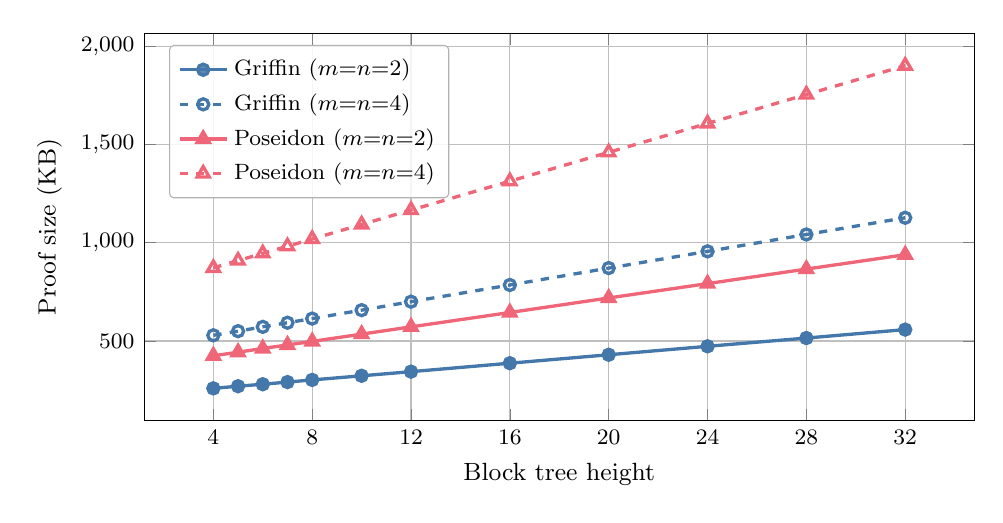
\begin{tikzpicture}
    \begin{axis}[
      xlabel={Block tree height},
      ylabel={Proof size (KB)},
      xtick={4,8,12,16,20,24,28,32},
      legend style={
        at={(0.03,0.97)},
        anchor=north west,
        font=\footnotesize,
        draw=gray!60,
        fill=white,
        fill opacity=0.85,
        text opacity=1,
        rounded corners=1.5pt,
        inner sep=3pt,
        row sep=1pt,
      },
      legend cell align={left},
      grid=both,
      grid style={line width=0.2pt, draw=gray!25},
      major grid style={line width=0.4pt, draw=gray!50},
      width=\columnwidth,
      height=6.5cm,
      x tick label style={font=\footnotesize},
      y tick label style={font=\footnotesize},
      xlabel style={font=\small},
      ylabel style={font=\small},
      every axis plot/.append style={line width=1.2pt},
      mark size=2pt,
    ]
      % Griffin m=n=2
      \addplot[tolblue, mark=*, solid] coordinates {
        (4,259) (5,270) (6,280) (7,291) (8,302)
        (10,323) (12,344) (16,387) (20,430) (24,473) (28,515) (32,558)
      };
      % Griffin m=n=4
      \addplot[tolblue, mark=o, mark options=solid, dashed] coordinates {
        (4,529) (5,550) (6,572) (7,593) (8,614)
        (10,657) (12,700) (16,785) (20,871) (24,956) (28,1042) (32,1127)
      };
      % Poseidon m=n=2
      \addplot[tolred, mark=triangle*, solid, mark size=2.5pt] coordinates {
        (4,425) (5,443) (6,462) (7,480) (8,498)
        (10,535) (12,572) (16,645) (20,719) (24,792) (28,866) (32,939)
      };
      % Poseidon m=n=4
      \addplot[tolred, mark=triangle, mark options=solid, dashed, mark size=2.5pt] coordinates {
        (4,872) (5,909) (6,946) (7,982) (8,1019)
        (10,1093) (12,1166) (16,1313) (20,1460) (24,1607) (28,1754) (32,1901)
      };
      \legend{Griffin ($m{=}n{=}2$), Griffin ($m{=}n{=}4$), Poseidon ($m{=}n{=}2$), Poseidon ($m{=}n{=}4$)}
    \end{axis}
  \end{tikzpicture}
  \caption{Client-side proof size as a function of block tree height $h$ using quaternary trees. The anonymity set size per epoch is $4^{h-1} \times 4096$ transactions.}
  \label{fig:proof-size-bench}
\end{figure}

\paragraph{Aggregator performance.}
\Cref{fig:aggregator-bench} breaks down the aggregator's block building time into four phases for varying numbers of transactions in a block.
First, user-submitted witness-instance pairs for transaction validity are \emph{verified} by checking public inputs and running the Nova verifier and decider.
The remaining three phases constitute a single IVC prove step per transaction:
the aggregator \emph{folds} the validated user pairs into an accumulated witness-instance pair,
\emph{executes} the step circuit,
and \emph{folds} the execution trace into the local witness-instance pair via \ac{IVC}.
All four phases scale linearly with the number of transactions.
Local instance folding dominates across all configurations, accounting for 51-60\% of the total runtime at 128 transactions, followed by user instance folding (19-21\%), step circuit synthesis (11-22\%), and validation (7-10\%).
At 128 transactions, the total aggregation time ranges from 34.0\,s (Griffin, $m{=}n{=}2$) to 45.5\,s (Poseidon, $m{=}n{=}4$).

\pgfplotsset{
  % Common axis options for the grouped stacked bar chart
  aggaxis/.style={
    ybar stacked,
    bar width=4pt,
    symbolic x coords={8,16,32,64,128},
    xtick=data,
    x tick label style={font=\footnotesize},
    y tick label style={font=\footnotesize},
    xlabel style={font=\small},
    ylabel style={font=\small},
    enlarge x limits=0.12,
    ymin=0, ymax=50,
    width=\columnwidth,
    height=7cm,
    ymajorgrids=true,
    grid style={line width=0.2pt, draw=gray!25},
    major grid style={line width=0.3pt, draw=gray!40},
  },
  %% Poseidon m=n=2: solid fill, solid border
  P2val/.style={fill=tolblue, draw=tolblue!80!black, line width=0.4pt},
  P2fu/.style={fill=tolgreen, draw=tolgreen!80!black, line width=0.4pt},
  P2syn/.style={fill=tolyellow, draw=tolyellow!80!black, line width=0.4pt},
  P2fl/.style={fill=tolred, draw=tolred!80!black, line width=0.4pt},
  %% Griffin m=n=2: no fill, solid colored border
  G2val/.style={fill=white, draw=tolblue, line width=0.5pt},
  G2fu/.style={fill=white, draw=tolgreen, line width=0.5pt},
  G2syn/.style={fill=white, draw=tolyellow!80!black, line width=0.5pt},
  G2fl/.style={fill=white, draw=tolred, line width=0.5pt},
  %% Poseidon m=n=4: solid fill, hatched
  P4val/.style={fill=tolblue, draw=tolblue!80!black, line width=0.4pt, postaction={pattern=north east lines, pattern color=white}},
  P4fu/.style={fill=tolgreen, draw=tolgreen!80!black, line width=0.4pt, postaction={pattern=north east lines, pattern color=white}},
  P4syn/.style={fill=tolyellow, draw=tolyellow!80!black, line width=0.4pt, postaction={pattern=north east lines, pattern color=white}},
  P4fl/.style={fill=tolred, draw=tolred!80!black, line width=0.4pt, postaction={pattern=north east lines, pattern color=white}},
  %% Griffin m=n=4: no fill, hatched
  G4val/.style={fill=white, draw=tolblue, line width=0.5pt, postaction={pattern=north east lines, pattern color=tolblue}},
  G4fu/.style={fill=white, draw=tolgreen, line width=0.5pt, postaction={pattern=north east lines, pattern color=tolgreen}},
  G4syn/.style={fill=white, draw=tolyellow!80!black, line width=0.5pt, postaction={pattern=north east lines, pattern color=tolyellow!80!black}},
  G4fl/.style={fill=white, draw=tolred, line width=0.5pt, postaction={pattern=north east lines, pattern color=tolred}},
}

\begin{figure}[!ht]
  \centering
  \begin{tikzpicture}
    %%% Axis 1: Poseidon m=n=2 (solid, leftmost)
    \begin{axis}[name=mainaxis, aggaxis, bar shift=-9pt,
      xlabel={Number of transactions}, ylabel={Time (s)},
    ]
      \addplot[P2val] coordinates {(8,0.212) (16,0.421) (32,0.850) (64,1.682) (128,3.363)};
      \addplot[P2fu] coordinates {(8,0.419) (16,0.884) (32,1.813) (64,3.908) (128,7.874)};
      \addplot[P2syn] coordinates {(8,0.267) (16,0.531) (32,1.035) (64,2.089) (128,4.197)};
      \addplot[P2fl] coordinates {(8,1.101) (16,2.496) (32,5.198) (64,10.558) (128,21.551)};
    \end{axis}
    %%% Axis 2: Griffin m=n=2 (no fill, solid border)
    \begin{axis}[aggaxis, bar shift=-3pt,
      axis x line=none, axis y line=none,
      xtick=\empty, ytick=\empty,
    ]
      \addplot[G2val] coordinates {(8,0.212) (16,0.421) (32,0.850) (64,1.682) (128,3.363)};
      \addplot[G2fu] coordinates {(8,0.423) (16,0.939) (32,1.774) (64,3.465) (128,7.230)};
      \addplot[G2syn] coordinates {(8,0.366) (16,0.707) (32,1.432) (64,2.853) (128,5.708)};
      \addplot[G2fl] coordinates {(8,0.918) (16,2.120) (32,4.226) (64,8.765) (128,17.638)};
    \end{axis}
    %%% Axis 3: Poseidon m=n=4 (solid fill, dashed border)
    \begin{axis}[aggaxis, bar shift=3pt,
      axis x line=none, axis y line=none,
      xtick=\empty, ytick=\empty,
    ]
      \addplot[P4val] coordinates {(8,0.212) (16,0.421) (32,0.850) (64,1.682) (128,3.363)};
      \addplot[P4fu] coordinates {(8,0.586) (16,1.034) (32,2.045) (64,4.235) (128,8.890)};
      \addplot[P4syn] coordinates {(8,0.360) (16,0.717) (32,1.434) (64,2.876) (128,5.761)};
      \addplot[P4fl] coordinates {(8,1.509) (16,3.257) (32,6.492) (64,13.318) (128,27.476)};
    \end{axis}
    %%% Axis 4: Griffin m=n=4 (no fill, dashed border)
    \begin{axis}[aggaxis, bar shift=9pt,
      axis x line=none, axis y line=none,
      xtick=\empty, ytick=\empty,
    ]
      \addplot[G4val] coordinates {(8,0.212) (16,0.421) (32,0.850) (64,1.682) (128,3.363)};
      \addplot[G4fu] coordinates {(8,0.453) (16,1.017) (32,1.808) (64,4.140) (128,7.663)};
      \addplot[G4syn] coordinates {(8,0.536) (16,1.078) (32,2.129) (64,4.285) (128,8.564)};
      \addplot[G4fl] coordinates {(8,1.048) (16,2.403) (32,4.787) (64,9.891) (128,20.031)};
    \end{axis}
    %%% Legend overlay (outside all axes to avoid symbolic coord issues)
    \node[anchor=north west, draw=gray!60, fill=white, rounded corners=1.5pt,
      inner sep=4pt]
      at ([xshift=4pt, yshift=-4pt]mainaxis.north west) {%
      \begin{tikzpicture}[
        txt/.style={anchor=mid west, font=\scriptsize, inner sep=0pt, outer sep=0pt},
      ]
        %% Left column: phase colors.  Right column: config patterns.
        %% sq side=0.25cm, col gap=0.12cm, row step=0.38cm, right col at x=3.1cm
        % Row 0
        \fill[fill=tolblue, draw=tolblue!80!black, line width=0.4pt]
          (0,0) rectangle (0.25,0.25);
        \node[txt] at (0.37, 0.125) {Verify user instances};
        \fill[fill=gray!70, draw=gray!50!black, line width=0.4pt]
          (3.1,0) rectangle (3.35,0.25);
        \node[txt] at (3.47, 0.125) {Poseidon ($m{=}n{=}2$)};
        % Row 1
        \fill[fill=tolgreen, draw=tolgreen!80!black, line width=0.4pt]
          (0,-0.38) rectangle (0.25,-0.13);
        \node[txt] at (0.37, -0.255) {Fold user instances};
        \fill[fill=white, draw=gray!50!black, line width=0.5pt]
          (3.1,-0.38) rectangle (3.35,-0.13);
        \node[txt] at (3.47, -0.255) {Griffin ($m{=}n{=}2$)};
        % Row 2
        \fill[fill=tolyellow, draw=tolyellow!80!black, line width=0.4pt]
          (0,-0.76) rectangle (0.25,-0.51);
        \node[txt] at (0.37, -0.635) {Execute step circuit};
        \fill[fill=gray!70, draw=gray!50!black, line width=0.4pt]
          (3.1,-0.76) rectangle (3.35,-0.51);
        \fill[pattern=north east lines, pattern color=white]
          (3.1,-0.76) rectangle (3.35,-0.51);
        \node[txt] at (3.47, -0.635) {Poseidon ($m{=}n{=}4$)};
        % Row 3
        \fill[fill=tolred, draw=tolred!80!black, line width=0.4pt]
          (0,-1.14) rectangle (0.25,-0.89);
        \node[txt] at (0.37, -1.015) {Fold local instances};
        \fill[fill=white, draw=gray!50!black, line width=0.5pt]
          (3.1,-1.14) rectangle (3.35,-0.89);
        \fill[pattern=north east lines, pattern color=gray!50!black]
          (3.1,-1.14) rectangle (3.35,-0.89);
        \node[txt] at (3.47, -1.015) {Griffin ($m{=}n{=}4$)};
      \end{tikzpicture}%
    };
  \end{tikzpicture}

  \caption{Aggregator-side block building time breakdown by phase.}
  \label{fig:aggregator-bench}
\end{figure}

\paragraph{Throughput.}
We consider regular transaction blocks where all senders have endorsed the committed \ac{UTXO} tree root.
The block header consists of the transaction, public key, and nullifier tree roots, all 32-byte values, totalling 96~bytes.
We assume MicroNova~\cite{SP:ZSCZ25} for the decider SNARK, with a compressed proof size of $\approx 12$\,KB.
We assume 4 inputs per transaction and fix nullifier sizes to 32~bytes.
We re-use Intmax2's proposed user-id size of ${\sim}\,4.15$~bytes, which makes it possible for \Protocol to accommodate more than the current world population.
Finally, we assume a blob target of 14 per \ac{L1} block, yielding $14 \times 131072 \approx 1835$\,KB of available blob space.

\begin{itemize}
  \item \textit{Centralized setting.} In the centralized setup, the aggregator does not post nullifier values.
The only per-transaction data is the sender's id (${\sim}\,4.15$~bytes).
Dividing the available blob space (minus proof and header overhead) by the per-transaction data, we get:
$$\frac{1835 \text{KB} - 12 \text{KB} - 0.096 \text{KB}}{{0.00415 \text{KB}}} \approx 439254$$
transactions per \ac{L1} block, or with a block time of 12\,s, $\approx 36604$ \ac{TPS}.


  \item \textit{Decentralized setting.} In the decentralized setup, the aggregator broadcasts along each sender id four input nullifier values.
This requires $4.15 + 4 \times 32 = 132.15$~bytes per transaction, resulting in ${\approx}\,13796$ transactions per \ac{L1} block, i.e.\ ${\approx}\,1149$ \ac{TPS}.
Note that one could also truncate nullifiers to 20~bytes, in which case $4.15 + 4 \times 20 = 84.15$~bytes per transaction is required, resulting in ${\approx}\,21668$ transactions per \ac{L1} block, i.e.\ ${\approx}\,1805$ \ac{TPS}.

\end{itemize}


\section*{Acknowledgments}

We thank Srinath Setty and Liam Eagen for 
conversations and comments which led to this paper. We thank \texttt{@arnaucube} and \texttt{@CPerezz} on GitHub for starting and maintaining early versions of \texttt{sonobe}.



\bibliographystyle{plain}
\bibliography{bib/abbrev3,bib/crypto,bibliography}

\end{document}
